\documentclass[11pt]{article}
\usepackage[a4paper,margin=25mm]{geometry}
\usepackage{amsmath,amssymb,amsthm,booktabs,tikz}
\usepackage[colorlinks=true,urlcolor=blue,citecolor=blue]{hyperref}
\hypersetup{pdftitle={Sharp thresholds for five-colour cube assemblies},pdfauthor={Jason Davies}}
\newtheorem{theorem}{Theorem}
\newtheorem{lemma}[theorem]{Lemma}
\newtheorem{proposition}[theorem]{Proposition}
\newtheorem{corollary}[theorem]{Corollary}
\theoremstyle{remark}
\newtheorem*{remark}{Remark}
\newcommand{\col}{\{0,1,2,3,4\}}
\newcommand{\mass}[2]{#1(#2)}
\title{Sharp thresholds for five-colour cube assemblies}
\author{Jason Davies}
\date{November 4, 2026}
\begin{document}
\maketitle
\begin{center}\small Editorial integration draft: companion mathematical appendix under consolidation.\end{center}
\begin{abstract}
We determine the least pool sizes guaranteeing a frame or a complete
$a\times b\times c$ box from unit cubes whose faces use all five colours
of a fixed palette, for every $a,b,c\ge2$. Proper rotations are allowed;
the target has monochromatic exterior faces using all five colours.
The frame threshold is $\max\{15,4(a+b+c)-16,2(a+b+c)+1\}$, and the
complete-box threshold is $\max\{abc,15,2(a+b+c)+1\}$.
Thus the frame threshold depends only on the sum of the side lengths,
and only three complete-box shapes can require spare sources.
The proof combines an elementary fifteen-cube corner theorem with Hall
arguments and a uniform three-variety obstruction. The corner proof uses
directed cuts, repeated-colour completions and geometric case analysis;
its longer cases are proved in a companion mathematical appendix. It completes the
five-colour frame column left open by Berkove, Eickemeyer and Schulman
(2018). The same threshold statements have a separate Lean verification, using
a certificate-based proof of the corner theorem. A fixed-size flow
formulation constructs assemblies in time linear in the explicit input
and output sizes. A secondary result, using additional finite checks, determines corner
thresholds when the number of source varieties is bounded.
\end{abstract}
\noindent\small\textit{AI transparency.} The research, code and manuscript were
developed using GPT-6-Astra (OpenAI), through Codex, under the author's
direction. This working manuscript has not received independent human peer
review; Section~\ref{sec:formal} states the formal verification scope.
\normalsize

\section{Introduction}
MacMahon's coloured-cube puzzles~\cite{MacMahon} ask when a collection of
face-coloured cubes can form a larger cube with monochromatic exterior
faces. Here every source and target uses all five colours of a fixed
palette. Proper rotations identify varieties; reflections are not allowed
as moves. Collections may contain repeated varieties, and touching interior
faces need not have equal colours.
For $a,b,c\ge2$, a \emph{frame} consists of the eight corners and the
noncorner positions on the twelve edges of an $a\times b\times c$ box.
It has $L=4(a+b+c)-16$ positions. Write $F_5(a,b,c)$ for the least pool
size guaranteeing a frame and $G_5(a,b,c)$ for the least pool size
guaranteeing a complete box. An assembly may use a subset of the pool;
its target colouring may depend on the collection.

\begin{theorem}[All cuboid thresholds]\label{thm:all-boxes}
For every integer $a,b,c\ge2$,
\[
 \begin{aligned}
 F_5(a,b,c)&=\max\{15,4(a+b+c)-16,2(a+b+c)+1\},\\
 G_5(a,b,c)&=\max\{abc,15,2(a+b+c)+1\}.
 \end{aligned}
\]
\end{theorem}
The frame threshold depends only on the sum $s=a+b+c$: it is $15$ for
$s=6,7$, $17$ for $s=8$, and the frame's own cardinality $4s-16$ for
$s\ge9$. Up to permuting sides, only three complete boxes can require
spare sources: $2\times2\times2$, $2\times2\times3$, and
$2\times2\times4$, whose thresholds are $15,15,17$.
The distinction between the two thresholds matters: a $2\times3\times3$
frame has sixteen positions and needs seventeen available sources,
whereas its complete box uses any eighteen sources without spares.
Table~\ref{tab:small-boxes} lists the smallest shapes; from $s=9$ on, both
thresholds equal the number of positions.
\begin{table}[ht]
\centering
\small
\begin{tabular}{c c c c c c}
\toprule
Box & $s$ & Frame positions & $F_5$ & Volume & $G_5$\\
\midrule
$2\times2\times2$ & 6 & 8 & \textbf{15} & 8 & \textbf{15}\\
$2\times2\times3$ & 7 & 12 & \textbf{15} & 12 & \textbf{15}\\
$2\times2\times4$ & 8 & 16 & \textbf{17} & 16 & \textbf{17}\\
$2\times3\times3$ & 8 & 16 & \textbf{17} & 18 & 18\\
$2\times2\times5$ & 9 & 20 & 20 & 20 & 20\\
$2\times3\times4$ & 9 & 20 & 20 & 24 & 24\\
$3\times3\times3$ & 9 & 20 & 20 & 27 & 27\\
\bottomrule
\end{tabular}
\caption{Thresholds for the smallest boxes. A bold entry exceeds the number
of positions: some collections with no spare sources fail.}
\label{tab:small-boxes}
\end{table}

For ordinary cubes, abbreviate $F_5(n)=F_5(n,n,n)$ and
$G_5(n)=G_5(n,n,n)$. The classification immediately gives the following.
\begin{corollary}[Ordinary cubes]\label{thm:frames}\label{thm:complete}
\[
 F_5(n)=\begin{cases}15,&n=2,\\12n-16,&n\ge3,\end{cases}
 \qquad G_5(n)=\max\{n^3,15\}\quad(n\ge2).
\]
In particular, any twenty sources form the frame of a $3\times3\times3$ cube, and any 27 form a
complete $3\times3\times3$ cube.
\end{corollary}

Berkove, Eickemeyer and Schulman~\cite[Section 8, Table 7]{BES} record
frame thresholds for palettes of two to six colours, leaving the
five-colour column open. Table~\ref{tab:palette-thresholds} inserts the
values proved here; the cuboid classification goes beyond that table.
\begin{table}[ht]
\centering
\small
\begin{tabular}{c c c c c c}
\toprule
Side length & 2 colours & 3 colours & 4 colours & \textbf{5 colours} & 6 colours\\
\midrule
$n=2$ & 11 & 23 & 11 & \textbf{15} & 24\\
$n=3$ & 20 & 35 & 20 & \textbf{20} & 24\\
$n\ge4$ & $12n-16$ & $16n-17$ & $12n-16$ & $\boldsymbol{12n-16}$ & $12n-16$\\
\bottomrule
\end{tabular}
\caption{Cube-frame thresholds. The five-colour column is proved here;
other columns are as recorded in~\cite[Table 7]{BES}.}
\label{tab:palette-thresholds}
\end{table}

We first prove the corner threshold independently of the extensions.
Write $N_5=F_5(2)=G_5(2)$.
\begin{theorem}[Corner threshold]\label{thm:main}
$N_5=15$.
\end{theorem}
An elementary fourteen-cube obstruction proves the lower bound.
For the upper bound, adjacent corner classes become directed cuts on five
colours, while opposite-repeat varieties become bidirected four-cycles.
Small matching constructions and repeated-colour arguments constrain a
hypothetical failure. Compression of disjoint cuts reduces the two-opposite
case to three geometric support families. Section~\ref{sec:elementary}
combines these ingredients into a direct fifteen-source proof; all necessary
longer cases are included in the companion mathematical appendix, submitted
as part of the proof rather than as optional computational material.

Section~\ref{sec:frames} establishes the shared geometry, including the
eight-plus-three missing-pair lemma independently of the corner theorem.
Section~\ref{sec:boxes} extends the corner input to all cuboids. A uniform
three-variety obstruction explains the two sixteen-position exceptions.
Section~\ref{sec:construction} gives a compressed flow algorithm, and
Section~\ref{sec:support} treats bounded numbers of source varieties using
separate finite geometric checks. The elementary-proof claim concerns the
main threshold classification. Section~\ref{sec:formal} distinguishes that
argument from the existing formal verification.

The side-length restriction is substantive. With a side of length one,
a source can meet two opposite exterior faces and expose four or more
faces at once. The corner-and-edge model and the completion by arbitrary
unused cubes then need replacement.

The accompanying repository contains the certificates, programs,
geometric audits and Lean sources.\footnote{\url{https://github.com/jasondavies/five-colour-cubes}.
A fixed review archive includes source checksums, the base Git revision and
bundled pinned project dependencies.}

The companion paper~\cite{FourToThree} considers four-colour sources and
targets using exactly three colours. It gives the sharp frame threshold
$16n-3$ for every side length $n\ge2$, with a classification of the largest
failing collections. The two developments share the palette-independent
geometry in the \texttt{colour-\allowbreak cubes-\allowbreak core} library~\cite{ColourCubes};
neither threshold theorem is used to prove the other.

\section{Geometry and Hall deficiencies}\label{sec:model}
Represent a cube by its colours on the faces
$(+x,-x,+y,-y,+z,-z)$ in a right-handed coordinate frame. A five-colour cube
has one repeated colour. There are 75 varieties: for each repeated colour,
three have its two faces opposite and twelve have them adjacent. In the
opposite case, the other four colours form two opposite pairs, giving three
possibilities. In the adjacent case, fix the two equal faces; the 24 orders
of the other colours are identified in pairs by the rotation exchanging
those equal faces. Thus there are 15 opposite-repeat varieties and 60
adjacent-repeat varieties. Each class is one orbit under colour permutations.

A corner type is the ordered triple of its incident face colours, modulo
cyclic permutation. Order the outward face normals positively, equivalently
read the triple counterclockwise from outside along the body diagonal.
This reverses the clockwise convention in~\cite{BES}, consistently on every
cube, and therefore preserves all matching and containment relations.
Repeated occurrences of a corner type are retained as distinct target
positions.

\begin{lemma}[Corner--rotation correspondence]\label{lem:corner}
A source cube fits a target corner by a proper rotation if and only if it
has the same cyclic corner type at some corner.
\end{lemma}
\begin{proof}
A proper rotation preserves the orientation of a corner frame, so it induces
a cyclic permutation of its three outward faces. Conversely, any two
positively oriented corner frames, with a prescribed cyclic alignment,
are related by a determinant-positive signed permutation of the coordinate
axes. This is a proper rotation of the cube.
\end{proof}
The palette-independent Lean version of this lemma is reused from the
shared \texttt{colour-\allowbreak cubes-\allowbreak core} library~\cite{ColourCubes}.

Fix a target $T$. Form a bipartite graph whose left vertices are its eight
corner positions and whose right vertices are the individual source copies.
A copy is adjacent to a position when it fits there. A matching covering
the eight positions is exactly a solution: each chosen copy can be rotated
independently, since interior faces are unrestricted. By Hall's
theorem~\cite{Hall}, failure is equivalent to a nonempty set $D$ of target
positions having fewer than $|D|$ neighbouring copies.

Index the varieties by $i=1,\ldots,75$, and let $x_i$ be their multiplicities.
For a set $S$ of varieties, write $x(S)=\sum_{i\in S}x_i$.
Let $N_T(D)$ be the varieties fitting at least one position of $D$. Then
failure of $T$ is equivalent to the existence of a cut
\begin{equation}\label{eq:hall}
  x(N_T(D))\le |D|-1,\qquad \varnothing\ne D\subseteq\{1,\ldots,8\}.
\end{equation}
There are 255 cuts per target, hence 19,125 cuts altogether.

\section{Shared geometric and matching tools}\label{sec:frames}
The corner and frame arguments share the following geometric and matching tools.
All statements in this section are independent of the corner threshold.
Lemmas~\ref{lem:cube-incidence} and~\ref{lem:transverse-corner} state the
shape-independent facts used in the directional bounds of
Section~\ref{sec:boxes}.
The following form of Hall's theorem isolates the matching step.

\begin{lemma}[Hall criterion with a matched subset]\label{lem:partial-matching}
Consider $L$ target positions and $N\ge L$ source copies. Suppose every
source misses at most $d$ positions. If a set $P_0$ of positions can be
matched to distinct copies, and every position outside $P_0$ has at least
$d$ neighbours, then all $L$ positions can be matched.
\end{lemma}
\begin{proof}
For a position set $D\subseteq P_0$, the given matching supplies $|D|$
neighbours. If $D\nsubseteq P_0$ and $|D|\le d$, a position in
$D\setminus P_0$ alone has at least $d$ neighbours. If $|D|>d$, every
source neighbours $D$, since none can miss all its positions. In each case
Hall's inequality holds.
\end{proof}

\begin{lemma}[Missing pairs and shared corners]\label{lem:cube-incidence}
Every five-colour variety has eight distinct cyclic corner types.
An adjacent-repeat variety lacks exactly one bichromatic edge type;
an opposite-repeat variety lacks exactly two, which are disjoint.
Two disjoint missing pairs determine a unique opposite-repeat variety.
If either of two varieties is opposite-repeat, they share at least two
corner types. A target has at most one monochromatic edge; each bichromatic
type occurs on at most two edges, and a doubled type contains the repeated
colour. Thus two disjoint bichromatic types account for at most three
geometric target edges.
\end{lemma}
\begin{proof}
A missing bichromatic pair occupies opposite singleton faces: if a colour
is repeated, a face of the other colour cannot be opposite both copies.
An adjacent-repeat variety has one opposite pair of singleton faces, and an
opposite-repeat variety has two. Two disjoint missing pairs specify two
opposite face pairs, leaving the fifth colour on the remaining pair,
which determines a unique variety.

For the shared-corner assertion, let the opposite-repeat variety repeat
$r$, with singleton opposite pairs $\{\alpha,\beta\}$ and
$\{\gamma,\delta\}$. It contains both cyclic orientations of each
$rxy$ with $x\in\{\alpha,\beta\}$ and $y\in\{\gamma,\delta\}$.
In the other variety, an $r$-face with no adjacent $r$-face has at least
three distinct colours around it. Their cyclic order crosses between the
two pairs at least twice, giving two shared corners. If its $r$-faces
are adjacent, the other neighbours of each form a path of three distinct
colours. Each path crosses between the pairs and gives a shared corner,
and these have different types. Corner counts are symmetric: a five-colour
variety has eight distinct cyclic corner types, since the only repeated
colour multisets occur at the two ends of an edge, in opposite cyclic orders.

Only the repeated colour can form a monochromatic edge. Two singleton
faces meet along at most one edge; hence a doubled bichromatic type
contains the repeated colour and occurs at most twice. Two disjoint types
cannot both contain that colour, proving the final bound.
\end{proof}

\begin{lemma}[A transverse edge forces a common corner]\label{lem:transverse-corner}
Let source and target both be adjacent-repeat varieties. If the source
lacks the type of a target edge not parallel to the target's monochromatic
edge, then it shares a corner type with the target.
\end{lemma}
\begin{proof}
Relabel the colours and rotate the target to $T=(0,1,0,2,3,4)$.
Its monochromatic edge is parallel to $z$.
The types occurring on edges transverse to the monochromatic edge are
$03,04,13,14,23,24$.  The proper half-turn interchanging the $x$- and
$y$-directions and reversing $z$, followed by the colour relabelling
$1\leftrightarrow2$, $3\leftrightarrow4$, fixes $T$ and pairs these types
as $(03,04)$, $(13,24)$, and $(14,23)$.  Thus three cases suffice.
For each missing type the source has its two colours on opposite faces.
The other three colours occur around that axis in one of two cyclic
orientations.  The three adjacent-repeat choices in each orientation
share six tricoloured corners.  Reading those common corners gives:
\[
\begin{array}{c|c|c}
\text{Missing type}&\text{Shared corners in one orientation}
 &\text{Shared corners in the other orientation}\\\hline
03&024,041&123\\
13&032&041,142\\
14&013,123&024
\end{array}
\]
Every entry is nonempty, so the source and target share a corner.
\end{proof}

For a bichromatic pair $\alpha\beta$, let $\mathcal H_{\alpha\beta}$ be the family of
varieties lacking that edge type.  In every such cube, $\alpha$ and $\beta$ are
opposite singleton faces.  The four faces around this axis use the other
three colours, one of them twice.  There are nine varieties in
$\mathcal H_{\alpha\beta}$: three opposite-repeat varieties $O_r$, and six
adjacent-repeat varieties $A_r^+$ and $A_r^-$, where $r$ is the repeated
colour.  The signs distinguish the two cyclic orientations of the three
distinct ring colours.  All three $A_r^+$ varieties share the same six
tricoloured corner types; all three $A_r^-$ varieties share the reverse
six types.

\begin{lemma}[The missing-pair corner array]\label{lem:fixed-missing-pair}
The eight corners of an opposite-repeat target $O_r\in\mathcal H_{\alpha\beta}$
form a $2\times2$ array with two positions per cell. Rows correspond to
the two unordered ring-colour pairs involving $r$, and columns to their
cyclic orientations. A source $O_r$ fits every cell; the other two
opposite-repeat varieties each fit one row; and the positive and negative
adjacent-repeat varieties fit the corresponding columns.
Consequently, every variety in $\mathcal H_{\alpha\beta}$ shares at least four
corner types with every opposite-repeat variety in that family.
\end{lemma}
\begin{proof}
Each cell contains one corner at each end of the $\alpha\beta$ axis.
Reading the ring colours gives the stated incidences. Figure~\ref{fig:ring-array}
shows the example $O_2=(0,1,2,2,3,4)$ in $\mathcal H_{01}$, with $+$
chosen to include $023$. Relabelling the three ring colours gives the
other two targets, and relabelling the palette gives every missing-pair
family. Cyclic rotations identify corner labels. In particular, the
two positions in each cell have identical source neighbourhoods.
\end{proof}

\begin{figure}[ht]
\centering
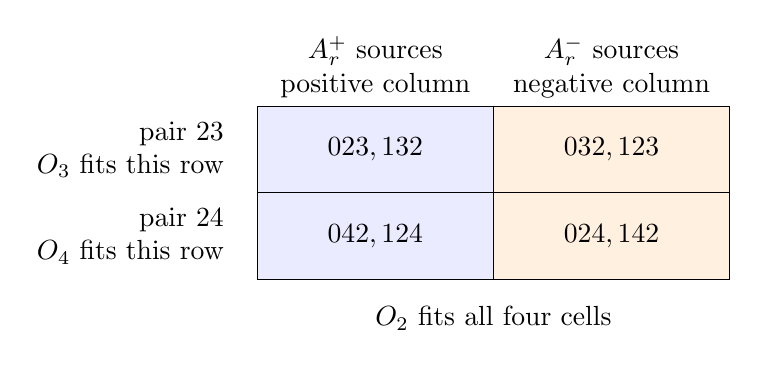
\begin{tikzpicture}[x=3cm,y=1.1cm]
\fill[blue!8] (0,0) rectangle (1,2);
\fill[orange!12] (1,0) rectangle (2,2);
\draw (0,0) rectangle (2,2);
\draw (1,0)--(1,2); \draw (0,1)--(2,1);
\node at (.5,1.5) {$023,132$};
\node at (1.5,1.5) {$032,123$};
\node at (.5,.5) {$042,124$};
\node at (1.5,.5) {$024,142$};
\node[align=center] at (.5,2.45) {$A_r^+$ sources\\positive column};
\node[align=center] at (1.5,2.45) {$A_r^-$ sources\\negative column};
\node[anchor=east,align=right] at (-.1,1.5) {pair $23$\\$O_3$ fits this row};
\node[anchor=east,align=right] at (-.1,.5) {pair $24$\\$O_4$ fits this row};
\node at (1,-.45) {$O_2$ fits all four cells};
\end{tikzpicture}
\caption{Corner array of $O_2$ in the family lacking $01$.
Each cell contains two target positions. Here $r\in\{2,3,4\}$;
all three adjacent-repeat sources of a given sign fit the same column.}
\label{fig:ring-array}
\end{figure}

\subsection{Signed corner projections}
Retain the family $\mathcal H_{\alpha\beta}$ from Lemma~\ref{lem:fixed-missing-pair},
with its opposite-repeat varieties and their $2\times2$ corner array.
Write $C(W)$ for the cyclic corner types of $W$.

\begin{lemma}[Corner projections onto a missing-pair family]\label{lem:thin-projections}
Fix a bichromatic pair $\alpha\beta$.  Let $C^+$ and $C^-$ be the two sets of six
tricoloured corner types shared by the three adjacent-repeat varieties of
the respective cyclic orientations in $\mathcal H_{\alpha\beta}$.  An
opposite-repeat variety in $\mathcal H_{\alpha\beta}$ has four corners in each set.
For a source $W\notin\mathcal H_{\alpha\beta}$, put
\[
 p(W)=|C(W)\cap C^+|,\qquad m(W)=|C(W)\cap C^-|.
\]
Then
\[
 (p(W),m(W))\in\{(4,0),(2,1),(1,2),(2,2),(0,4)\}.
\]
\end{lemma}

\begin{proof}
Relabel the poles as $0,1$ and the ring colours as $2,3,4$.  Choose the
positive orientation so that
\[
 C^+=\{023,034,042,124,132,143\},\qquad
 C^-=\{024,032,043,123,134,142\}.
\]
Triples denote cyclic classes; face order is $(+x,-x,+y,-y,+z,-z)$.  The following table gives representatives of
all geometric cases outside $\mathcal H_{01}$, up to a colour permutation
preserving the pole pair and a simultaneous reflection, which may exchange
$C^+$ and $C^-$.  Such a reflection is only a symmetry of this incidence
calculation, not an allowed assembly move.
\[
\begin{array}{c|cc}
 W&p(W)&m(W)\\\hline
 (0,0,1,2,3,4)&2&2\\
 (0,1,0,2,3,4)&0&4\\
 (0,2,0,3,1,4)&2&1\\
 (0,2,1,2,3,4)&0&4\\
 (0,2,1,3,2,4)&2&1\\
 (0,2,1,3,4,4)&2&2
\end{array}
\]
To see that these cases exhaust the possibilities, first suppose a pole
colour is repeated.  Its two faces are either opposite, or adjacent; in
the latter case the other pole is opposite one repeated face or adjacent
to both.  If a ring colour is repeated, the two pole faces must be
adjacent, since otherwise $W$ belongs to $\mathcal H_{01}$.  Fix them at
$x^+$ and $y^+$.  Among the remaining faces $x^-,y^-,z^+,z^-$, an opposite
repeated pair is $z^+,z^-$.  An adjacent repeated pair is either $x^-,y^-$,
or one of $x^-,y^-$ together with one of $z^+,z^-$.  These are the final
three rows.

Each entry follows by reading the eight corners of the displayed cube.
The projections of the nine family
varieties themselves are $(6,0),(0,6)$, and $(4,4)$, as follows directly
from their ring descriptions.
\end{proof}

\begin{lemma}[Compatibility for a thin frame]\label{lem:thin-compatibility}
Choose an orientation of a five-colour target for a $2\times2\times3$
frame such that its four noncorner edge positions are bichromatic.
Every source cube fits at least four of the twelve positions.
\end{lemma}

\begin{proof}
If either source or target is opposite-repeat,
Lemma~\ref{lem:cube-incidence} gives two shared corners.
The four parallel bichromatic edges have either four distinct types or
two types occurring twice each. In the latter case both contain the
target's repeated colour. The source's missing pairs are disjoint, so
it fits at least two of these edges, giving four compatible positions.

If both varieties are adjacent-repeat, the four parallel edge types are
distinct and transverse to the monochromatic edge. The source fits either
all four, or at least three and a corner by
Lemma~\ref{lem:transverse-corner}. Again it fits four positions.
\end{proof}

\subsection{Eight family cubes and three arbitrary additions}

% Analytic lemma for the 2 x 2 x 3 five-colour problem.

\begin{lemma}[Eight cubes with a common missing pair]\label{lem:eight-common-missing}
Eight cubes from $\mathcal H_{\alpha\beta}$, together with any three additional
five-colour cubes, have a corner solution whose target belongs to
$\mathcal H_{\alpha\beta}$.
\end{lemma}

\begin{proof}
Let $O,P,Q$ count the opposite-repeat, positive
adjacent-repeat, and negative adjacent-repeat copies among the chosen eight.
Thus $O+P+Q=8$; $C^+$ and $C^-$ are as in Lemma~\ref{lem:thin-projections}.

If $O+\min(P,Q)\ge4$, the $2\times2$ Hall argument gives an
opposite-repeat corner solution from these eight copies alone. Explicitly,
choose $O_r$ whose opposite-repeat multiplicity is maximal. Each cell has
at least $O/2+\min(P,Q)\ge2$ neighbours, each row has at least
$8-O/2\ge4$, and each column has at least $O+\min(P,Q)\ge4$.
Every other nonempty union of cells has all eight copies as neighbours.

Otherwise exchange the signs so that $O+Q\le3$. Put
$\kappa=O+Q=8-P$, so $P\ge5$ and $0\le \kappa\le3$.
Some positive variety $A_r^+$ occurs at least twice. If its eight
corners have a matching among all eleven copies, we are done. Otherwise,
choose a deficient Hall set $D$ of its corners. The two copies of
$A_r^+$ fit every corner, so $|D|\ge3$ and $D$ contains a tricoloured
corner. All $P$ positive copies are therefore neighbours of $D$.
Let $R$ be its other neighbours and put $U=C^+\setminus D$, $u=|U|$.
Since $|D|+u\le8$,
\[
 P+|R|<|D|\le8-u,\qquad |R|+u\le \kappa-1.
\]
Remove the $P$ positive copies and the copies in $R$. Every surviving
copy has all its positive corners in $U$, and $u\le2$.

Every family opposite-repeat variety has four corners in $C^+$, so no
such chosen copy remains. At least
\[
 \kappa-|R|\ge u+1
\]
of the chosen nonpositive copies remain, and all of them are negative
adjacent-repeat copies. Each fits every corner in $C^-$. The remaining
pool has at least
\[
 \kappa+3-|R|\ge4+u
\]
copies.

Lemma~\ref{lem:thin-projections} gives the following implications for every source:
\[
\begin{array}{c|ccc}
 |C(W)\cap C^+|\le u &u=0&u=1&u=2\\\hline
 |C(W)\cap C^-|\ge&4&2&1.
\end{array}
\]
Indeed, the family varieties have projection sizes $(6,0),(0,6),(4,4)$,
and every variety outside the family has one of
$(4,0),(2,1),(1,2),(2,2),(0,4)$.

Partition $C^-$ into three pairs, indexed by the unordered pairs of ring
colours. The negative half of each family opposite-repeat target is the
union of two of these pairs. We will match one such four-position half
using the remaining pool, then use four positive copies for its positive
half.

Let $j$ be the number of negative-family copies in the remaining pool;
thus $j\ge u+1$. If $j\ge4$, the conclusion is immediate. If $j=3$,
another remaining copy fits at least one negative corner; choose a target
whose negative half contains it and fill the other three positions with
negative-family copies.

If $j=2$, then $u\le1$. Two other remaining copies each fit at least two
negative corners, so they can be assigned distinct ones. Any two negative
corners lie in the union of two of the three pairs. Choose the corresponding
opposite-repeat target and fill its other two negative positions with the
two negative-family copies.

Finally, if $j=1$, then $u=0$, and there are at least three other copies,
each fitting at least four of the six negative corners. Choose one of
these copies $W$. Some union of two of the three pairs contains at least
three of its negative corners. In that four-position half, every other
copy fits at least two positions. Hence $W$ and any two other copies can
be matched to three distinct positions: two copies have at least two
neighbours, and all three together have at least three. The one
negative-family copy fills the fourth position.

In every case we obtain the negative half of an opposite-repeat target
in $\mathcal H_{\alpha\beta}$. Four of the $P\ge5$ positive copies fill its
positive half. The positive copies used here are disjoint from the surviving pool. This proves the lemma.
\end{proof}




\section{An elementary fourteen-cube obstruction}\label{sec:lower}
Consider four copies of $A$, five of $B$, and five of $C$, where
\[
 A=(0,0,1,2,3,4),\quad B=(0,1,2,3,2,4),\quad C=(0,3,1,2,4,1).
\]
Their corner types are shown below. Triples denote cyclic classes; the last
column counts positions whose type occurs in neither of the other varieties.
\begin{center}
\begin{tabular}{clc}
\toprule
Variety & Corner types & Private positions\\
\midrule
$A$ & $013,014,023,024,031,032,041,042$ & 5\\
$B$ & $022,023,034,042,122,124,132,143$ & 6\\
$C$ & $011,014,021,042,113,123,134,243$ & 6\\
\bottomrule
\end{tabular}
\end{center}
\begin{lemma}\label{lem:lower}
The collection $4A+5B+5C$ has no five-colour solution.
\end{lemma}
\begin{proof}
A solvable target must have every corner type in the displayed union.
Its only two-colour types are $022,122,011,113$. An adjacent-repeat target
therefore repeats either colour 2, with types $022,122$, or colour 1,
with types $011,113$. In either case these two corners determine the colours
on the faces at the ends of the repeated-colour edge. The two orders of the
remaining colours give a mirror pair: $B$ and its mirror, or $C$ and its
mirror. The mirror of $B$ requires $043$, and the mirror of $C$ requires
$012$; both types are absent. Only $B,C$ remain.

An opposite-repeat target requires both cyclic orientations of each corner
triple. The unordered triples with both orientations in the union are
\[
  013,014,023,024,123,134.
\]
If its repeated colour is $r$, delete $r$ from the four triples containing
it. The remaining pairs must form a $K_{2,2}$ on the other four colours:
choose one face from each of their two opposite pairs. Colours 2 and 4
occur in fewer than four listed triples. For $r=1$ or $r=3$, the four pairs
have degree sequence $(3,2,2,1)$, so do not form $K_{2,2}$. For $r=0$, the
pairs are $13,14,23,24$, forcing opposite pairs $\{1,2\}$ and $\{3,4\}$.
This is $A$.

Thus only $A,B,C$ can be targets. Their private positions require respectively
at least five, six and six copies of the corresponding variety, exceeding
the available four, five and five copies (Figure~\ref{fig:obstruction}).
None is solvable.
\end{proof}

\begin{figure}[ht]
\centering
% Generated by scripts/generate_five_colour_figure.py; do not edit.
\definecolor{cube0}{HTML}{E69F00}
\definecolor{cube1}{HTML}{56B4E9}
\definecolor{cube2}{HTML}{009E73}
\definecolor{cube3}{HTML}{F0E442}
\definecolor{cube4}{HTML}{CC79A7}
\begin{tikzpicture}[x=0.198mm,y=-0.198mm]
\path[use as bounding box] (0,0) rectangle (800,470);
\node[anchor=center,inner sep=0pt,outer sep=0pt,text=black!93,font={\sffamily\fontsize{10}{12}\selectfont\bfseries}] at (72,22) {Collection};
\node[anchor=center,inner sep=0pt,outer sep=0pt,text=black!93,font={\sffamily\fontsize{10}{12}\selectfont\bfseries}] at (372,22) {Corner types of each variety};
\node[anchor=west,inner sep=0pt,outer sep=0pt,text=black!93,font={\sffamily\fontsize{10}{12}\selectfont\bfseries}] at (604,22) {Why it fails};
\draw[draw=black!20,line width=0.674pt] (16,40) -- (784,40);
\draw[fill=cube3,draw=black!87,line join=round,line width=0.674pt] (48,54) -- (72,54) -- (72,78) -- (48,78) -- cycle;
\node[anchor=center,inner sep=0pt,outer sep=0pt,text=black!93,font={\sffamily\fontsize{10}{12}\selectfont}] at (60,66) {3};
\draw[fill=cube2,draw=black!87,line join=round,line width=0.674pt] (24,78) -- (48,78) -- (48,102) -- (24,102) -- cycle;
\node[anchor=center,inner sep=0pt,outer sep=0pt,text=black!93,font={\sffamily\fontsize{10}{12}\selectfont}] at (36,90) {2};
\draw[fill=cube0,draw=black!87,line join=round,line width=0.674pt] (48,78) -- (72,78) -- (72,102) -- (48,102) -- cycle;
\node[anchor=center,inner sep=0pt,outer sep=0pt,text=black!93,font={\sffamily\fontsize{10}{12}\selectfont}] at (60,90) {0};
\draw[fill=cube1,draw=black!87,line join=round,line width=0.674pt] (72,78) -- (96,78) -- (96,102) -- (72,102) -- cycle;
\node[anchor=center,inner sep=0pt,outer sep=0pt,text=black!93,font={\sffamily\fontsize{10}{12}\selectfont}] at (84,90) {1};
\draw[fill=cube0,draw=black!87,line join=round,line width=0.674pt] (96,78) -- (120,78) -- (120,102) -- (96,102) -- cycle;
\node[anchor=center,inner sep=0pt,outer sep=0pt,text=black!93,font={\sffamily\fontsize{10}{12}\selectfont}] at (108,90) {0};
\draw[fill=cube4,draw=black!87,line join=round,line width=0.674pt] (48,102) -- (72,102) -- (72,126) -- (48,126) -- cycle;
\node[anchor=center,inner sep=0pt,outer sep=0pt,text=black!93,font={\sffamily\fontsize{10}{12}\selectfont}] at (60,114) {4};
\node[anchor=center,inner sep=0pt,outer sep=0pt,text=black!93,font={\sffamily\fontsize{10}{12}\selectfont\bfseries}] at (72,148) {4 \(\times\) A};
\node[anchor=center,inner sep=0pt,outer sep=0pt,text=black!93,font={\sffamily\fontsize{9}{10.8}\selectfont}] at (72,170) {001234};
\draw[fill=cube0,draw=black!87,line join=round,line width=0.674pt] (180,96) -- (162.679,86) -- (162.679,106) -- (180,116) -- cycle;
\node[anchor=center,inner sep=0pt,outer sep=0pt,text=black!93,font={\sffamily\fontsize{8}{9.6}\selectfont}] at (171.34,101) {0};
\draw[fill=cube1,draw=black!87,line join=round,line width=0.674pt] (180,96) -- (180,116) -- (197.321,106) -- (197.321,86) -- cycle;
\node[anchor=center,inner sep=0pt,outer sep=0pt,text=black!93,font={\sffamily\fontsize{8}{9.6}\selectfont}] at (188.66,101) {1};
\draw[fill=cube3,draw=black!87,line join=round,line width=0.674pt] (180,96) -- (197.321,86) -- (180,76) -- (162.679,86) -- cycle;
\node[anchor=center,inner sep=0pt,outer sep=0pt,text=black!93,font={\sffamily\fontsize{8}{9.6}\selectfont}] at (180,86) {3};
\node[anchor=center,inner sep=0pt,outer sep=0pt,text=black!93,font={\sffamily\fontsize{9}{10.8}\selectfont}] at (180,131) {013};
\draw[fill=cube0,draw=black!87,line join=round,line width=0.674pt] (234,96) -- (216.679,86) -- (216.679,106) -- (234,116) -- cycle;
\node[anchor=center,inner sep=0pt,outer sep=0pt,text=black!93,font={\sffamily\fontsize{8}{9.6}\selectfont}] at (225.34,101) {0};
\draw[fill=cube2,draw=black!87,line join=round,line width=0.674pt] (234,96) -- (234,116) -- (251.321,106) -- (251.321,86) -- cycle;
\node[anchor=center,inner sep=0pt,outer sep=0pt,text=black!93,font={\sffamily\fontsize{8}{9.6}\selectfont}] at (242.66,101) {2};
\draw[fill=cube4,draw=black!87,line join=round,line width=0.674pt] (234,96) -- (251.321,86) -- (234,76) -- (216.679,86) -- cycle;
\node[anchor=center,inner sep=0pt,outer sep=0pt,text=black!93,font={\sffamily\fontsize{8}{9.6}\selectfont}] at (234,86) {4};
\node[anchor=center,inner sep=0pt,outer sep=0pt,text=black!93,font={\sffamily\fontsize{9}{10.8}\selectfont}] at (234,131) {024};
\draw[fill=cube0,draw=black!87,line join=round,line width=0.674pt] (288,96) -- (270.679,86) -- (270.679,106) -- (288,116) -- cycle;
\node[anchor=center,inner sep=0pt,outer sep=0pt,text=black!93,font={\sffamily\fontsize{8}{9.6}\selectfont}] at (279.34,101) {0};
\draw[fill=cube3,draw=black!87,line join=round,line width=0.674pt] (288,96) -- (288,116) -- (305.321,106) -- (305.321,86) -- cycle;
\node[anchor=center,inner sep=0pt,outer sep=0pt,text=black!93,font={\sffamily\fontsize{8}{9.6}\selectfont}] at (296.66,101) {3};
\draw[fill=cube1,draw=black!87,line join=round,line width=0.674pt] (288,96) -- (305.321,86) -- (288,76) -- (270.679,86) -- cycle;
\node[anchor=center,inner sep=0pt,outer sep=0pt,text=black!93,font={\sffamily\fontsize{8}{9.6}\selectfont}] at (288,86) {1};
\node[anchor=center,inner sep=0pt,outer sep=0pt,text=black!93,font={\sffamily\fontsize{9}{10.8}\selectfont}] at (288,131) {031};
\draw[fill=cube0,draw=black!87,line join=round,line width=0.674pt] (342,96) -- (324.679,86) -- (324.679,106) -- (342,116) -- cycle;
\node[anchor=center,inner sep=0pt,outer sep=0pt,text=black!93,font={\sffamily\fontsize{8}{9.6}\selectfont}] at (333.34,101) {0};
\draw[fill=cube3,draw=black!87,line join=round,line width=0.674pt] (342,96) -- (342,116) -- (359.321,106) -- (359.321,86) -- cycle;
\node[anchor=center,inner sep=0pt,outer sep=0pt,text=black!93,font={\sffamily\fontsize{8}{9.6}\selectfont}] at (350.66,101) {3};
\draw[fill=cube2,draw=black!87,line join=round,line width=0.674pt] (342,96) -- (359.321,86) -- (342,76) -- (324.679,86) -- cycle;
\node[anchor=center,inner sep=0pt,outer sep=0pt,text=black!93,font={\sffamily\fontsize{8}{9.6}\selectfont}] at (342,86) {2};
\node[anchor=center,inner sep=0pt,outer sep=0pt,text=black!93,font={\sffamily\fontsize{9}{10.8}\selectfont}] at (342,131) {032};
\draw[fill=cube0,draw=black!87,line join=round,line width=0.674pt] (396,96) -- (378.679,86) -- (378.679,106) -- (396,116) -- cycle;
\node[anchor=center,inner sep=0pt,outer sep=0pt,text=black!93,font={\sffamily\fontsize{8}{9.6}\selectfont}] at (387.34,101) {0};
\draw[fill=cube4,draw=black!87,line join=round,line width=0.674pt] (396,96) -- (396,116) -- (413.321,106) -- (413.321,86) -- cycle;
\node[anchor=center,inner sep=0pt,outer sep=0pt,text=black!93,font={\sffamily\fontsize{8}{9.6}\selectfont}] at (404.66,101) {4};
\draw[fill=cube1,draw=black!87,line join=round,line width=0.674pt] (396,96) -- (413.321,86) -- (396,76) -- (378.679,86) -- cycle;
\node[anchor=center,inner sep=0pt,outer sep=0pt,text=black!93,font={\sffamily\fontsize{8}{9.6}\selectfont}] at (396,86) {1};
\node[anchor=center,inner sep=0pt,outer sep=0pt,text=black!93,font={\sffamily\fontsize{9}{10.8}\selectfont}] at (396,131) {041};
\draw[fill=cube0!30,draw=black!40,line join=round,line width=0.674pt] (450,96) -- (432.679,86) -- (432.679,106) -- (450,116) -- cycle;
\node[anchor=center,inner sep=0pt,outer sep=0pt,text=black!60,font={\sffamily\fontsize{8}{9.6}\selectfont}] at (441.34,101) {0};
\draw[fill=cube1!30,draw=black!40,line join=round,line width=0.674pt] (450,96) -- (450,116) -- (467.321,106) -- (467.321,86) -- cycle;
\node[anchor=center,inner sep=0pt,outer sep=0pt,text=black!60,font={\sffamily\fontsize{8}{9.6}\selectfont}] at (458.66,101) {1};
\draw[fill=cube4!30,draw=black!40,line join=round,line width=0.674pt] (450,96) -- (467.321,86) -- (450,76) -- (432.679,86) -- cycle;
\node[anchor=center,inner sep=0pt,outer sep=0pt,text=black!60,font={\sffamily\fontsize{8}{9.6}\selectfont}] at (450,86) {4};
\node[anchor=center,inner sep=0pt,outer sep=0pt,text=black!60,font={\sffamily\fontsize{9}{10.8}\selectfont}] at (450,131) {014};
\draw[fill=cube0!30,draw=black!40,line join=round,line width=0.674pt] (504,96) -- (486.679,86) -- (486.679,106) -- (504,116) -- cycle;
\node[anchor=center,inner sep=0pt,outer sep=0pt,text=black!60,font={\sffamily\fontsize{8}{9.6}\selectfont}] at (495.34,101) {0};
\draw[fill=cube2!30,draw=black!40,line join=round,line width=0.674pt] (504,96) -- (504,116) -- (521.321,106) -- (521.321,86) -- cycle;
\node[anchor=center,inner sep=0pt,outer sep=0pt,text=black!60,font={\sffamily\fontsize{8}{9.6}\selectfont}] at (512.66,101) {2};
\draw[fill=cube3!30,draw=black!40,line join=round,line width=0.674pt] (504,96) -- (521.321,86) -- (504,76) -- (486.679,86) -- cycle;
\node[anchor=center,inner sep=0pt,outer sep=0pt,text=black!60,font={\sffamily\fontsize{8}{9.6}\selectfont}] at (504,86) {3};
\node[anchor=center,inner sep=0pt,outer sep=0pt,text=black!60,font={\sffamily\fontsize{9}{10.8}\selectfont}] at (504,131) {023};
\draw[fill=cube0!30,draw=black!40,line join=round,line width=0.674pt] (558,96) -- (540.679,86) -- (540.679,106) -- (558,116) -- cycle;
\node[anchor=center,inner sep=0pt,outer sep=0pt,text=black!60,font={\sffamily\fontsize{8}{9.6}\selectfont}] at (549.34,101) {0};
\draw[fill=cube4!30,draw=black!40,line join=round,line width=0.674pt] (558,96) -- (558,116) -- (575.321,106) -- (575.321,86) -- cycle;
\node[anchor=center,inner sep=0pt,outer sep=0pt,text=black!60,font={\sffamily\fontsize{8}{9.6}\selectfont}] at (566.66,101) {4};
\draw[fill=cube2!30,draw=black!40,line join=round,line width=0.674pt] (558,96) -- (575.321,86) -- (558,76) -- (540.679,86) -- cycle;
\node[anchor=center,inner sep=0pt,outer sep=0pt,text=black!60,font={\sffamily\fontsize{8}{9.6}\selectfont}] at (558,86) {2};
\node[anchor=center,inner sep=0pt,outer sep=0pt,text=black!60,font={\sffamily\fontsize{9}{10.8}\selectfont}] at (558,131) {042};
\draw[draw=black!87,line width=0.787pt] (158,144) -- (158,150) -- (418,150) -- (418,144);
\node[anchor=center,inner sep=0pt,outer sep=0pt,text=black!93,font={\sffamily\fontsize{9}{10.8}\selectfont\bfseries}] at (288,168) {5 private};
\node[anchor=west,inner sep=0pt,outer sep=0pt,text=black!93,font={\sffamily\fontsize{10}{12}\selectfont}] at (604,86) {5 corners need A;};
\node[anchor=west,inner sep=0pt,outer sep=0pt,text=black!93,font={\sffamily\fontsize{10}{12}\selectfont\bfseries}] at (604,112) {only 4 copies.};
\draw[draw=black!20,line width=0.674pt] (16,180) -- (784,180);
\draw[fill=cube2,draw=black!87,line join=round,line width=0.674pt] (48,194) -- (72,194) -- (72,218) -- (48,218) -- cycle;
\node[anchor=center,inner sep=0pt,outer sep=0pt,text=black!93,font={\sffamily\fontsize{10}{12}\selectfont}] at (60,206) {2};
\draw[fill=cube3,draw=black!87,line join=round,line width=0.674pt] (24,218) -- (48,218) -- (48,242) -- (24,242) -- cycle;
\node[anchor=center,inner sep=0pt,outer sep=0pt,text=black!93,font={\sffamily\fontsize{10}{12}\selectfont}] at (36,230) {3};
\draw[fill=cube0,draw=black!87,line join=round,line width=0.674pt] (48,218) -- (72,218) -- (72,242) -- (48,242) -- cycle;
\node[anchor=center,inner sep=0pt,outer sep=0pt,text=black!93,font={\sffamily\fontsize{10}{12}\selectfont}] at (60,230) {0};
\draw[fill=cube2,draw=black!87,line join=round,line width=0.674pt] (72,218) -- (96,218) -- (96,242) -- (72,242) -- cycle;
\node[anchor=center,inner sep=0pt,outer sep=0pt,text=black!93,font={\sffamily\fontsize{10}{12}\selectfont}] at (84,230) {2};
\draw[fill=cube1,draw=black!87,line join=round,line width=0.674pt] (96,218) -- (120,218) -- (120,242) -- (96,242) -- cycle;
\node[anchor=center,inner sep=0pt,outer sep=0pt,text=black!93,font={\sffamily\fontsize{10}{12}\selectfont}] at (108,230) {1};
\draw[fill=cube4,draw=black!87,line join=round,line width=0.674pt] (48,242) -- (72,242) -- (72,266) -- (48,266) -- cycle;
\node[anchor=center,inner sep=0pt,outer sep=0pt,text=black!93,font={\sffamily\fontsize{10}{12}\selectfont}] at (60,254) {4};
\node[anchor=center,inner sep=0pt,outer sep=0pt,text=black!93,font={\sffamily\fontsize{10}{12}\selectfont\bfseries}] at (72,288) {5 \(\times\) B};
\node[anchor=center,inner sep=0pt,outer sep=0pt,text=black!93,font={\sffamily\fontsize{9}{10.8}\selectfont}] at (72,310) {012324};
\draw[fill=cube0,draw=black!87,line join=round,line width=0.674pt] (180,236) -- (162.679,226) -- (162.679,246) -- (180,256) -- cycle;
\node[anchor=center,inner sep=0pt,outer sep=0pt,text=black!93,font={\sffamily\fontsize{8}{9.6}\selectfont}] at (171.34,241) {0};
\draw[fill=cube2,draw=black!87,line join=round,line width=0.674pt] (180,236) -- (180,256) -- (197.321,246) -- (197.321,226) -- cycle;
\node[anchor=center,inner sep=0pt,outer sep=0pt,text=black!93,font={\sffamily\fontsize{8}{9.6}\selectfont}] at (188.66,241) {2};
\draw[fill=cube2,draw=black!87,line join=round,line width=0.674pt] (180,236) -- (197.321,226) -- (180,216) -- (162.679,226) -- cycle;
\node[anchor=center,inner sep=0pt,outer sep=0pt,text=black!93,font={\sffamily\fontsize{8}{9.6}\selectfont}] at (180,226) {2};
\node[anchor=center,inner sep=0pt,outer sep=0pt,text=black!93,font={\sffamily\fontsize{9}{10.8}\selectfont}] at (180,271) {022};
\draw[fill=cube0,draw=black!87,line join=round,line width=0.674pt] (234,236) -- (216.679,226) -- (216.679,246) -- (234,256) -- cycle;
\node[anchor=center,inner sep=0pt,outer sep=0pt,text=black!93,font={\sffamily\fontsize{8}{9.6}\selectfont}] at (225.34,241) {0};
\draw[fill=cube3,draw=black!87,line join=round,line width=0.674pt] (234,236) -- (234,256) -- (251.321,246) -- (251.321,226) -- cycle;
\node[anchor=center,inner sep=0pt,outer sep=0pt,text=black!93,font={\sffamily\fontsize{8}{9.6}\selectfont}] at (242.66,241) {3};
\draw[fill=cube4,draw=black!87,line join=round,line width=0.674pt] (234,236) -- (251.321,226) -- (234,216) -- (216.679,226) -- cycle;
\node[anchor=center,inner sep=0pt,outer sep=0pt,text=black!93,font={\sffamily\fontsize{8}{9.6}\selectfont}] at (234,226) {4};
\node[anchor=center,inner sep=0pt,outer sep=0pt,text=black!93,font={\sffamily\fontsize{9}{10.8}\selectfont}] at (234,271) {034};
\draw[fill=cube1,draw=black!87,line join=round,line width=0.674pt] (288,236) -- (270.679,226) -- (270.679,246) -- (288,256) -- cycle;
\node[anchor=center,inner sep=0pt,outer sep=0pt,text=black!93,font={\sffamily\fontsize{8}{9.6}\selectfont}] at (279.34,241) {1};
\draw[fill=cube2,draw=black!87,line join=round,line width=0.674pt] (288,236) -- (288,256) -- (305.321,246) -- (305.321,226) -- cycle;
\node[anchor=center,inner sep=0pt,outer sep=0pt,text=black!93,font={\sffamily\fontsize{8}{9.6}\selectfont}] at (296.66,241) {2};
\draw[fill=cube2,draw=black!87,line join=round,line width=0.674pt] (288,236) -- (305.321,226) -- (288,216) -- (270.679,226) -- cycle;
\node[anchor=center,inner sep=0pt,outer sep=0pt,text=black!93,font={\sffamily\fontsize{8}{9.6}\selectfont}] at (288,226) {2};
\node[anchor=center,inner sep=0pt,outer sep=0pt,text=black!93,font={\sffamily\fontsize{9}{10.8}\selectfont}] at (288,271) {122};
\draw[fill=cube1,draw=black!87,line join=round,line width=0.674pt] (342,236) -- (324.679,226) -- (324.679,246) -- (342,256) -- cycle;
\node[anchor=center,inner sep=0pt,outer sep=0pt,text=black!93,font={\sffamily\fontsize{8}{9.6}\selectfont}] at (333.34,241) {1};
\draw[fill=cube2,draw=black!87,line join=round,line width=0.674pt] (342,236) -- (342,256) -- (359.321,246) -- (359.321,226) -- cycle;
\node[anchor=center,inner sep=0pt,outer sep=0pt,text=black!93,font={\sffamily\fontsize{8}{9.6}\selectfont}] at (350.66,241) {2};
\draw[fill=cube4,draw=black!87,line join=round,line width=0.674pt] (342,236) -- (359.321,226) -- (342,216) -- (324.679,226) -- cycle;
\node[anchor=center,inner sep=0pt,outer sep=0pt,text=black!93,font={\sffamily\fontsize{8}{9.6}\selectfont}] at (342,226) {4};
\node[anchor=center,inner sep=0pt,outer sep=0pt,text=black!93,font={\sffamily\fontsize{9}{10.8}\selectfont}] at (342,271) {124};
\draw[fill=cube1,draw=black!87,line join=round,line width=0.674pt] (396,236) -- (378.679,226) -- (378.679,246) -- (396,256) -- cycle;
\node[anchor=center,inner sep=0pt,outer sep=0pt,text=black!93,font={\sffamily\fontsize{8}{9.6}\selectfont}] at (387.34,241) {1};
\draw[fill=cube3,draw=black!87,line join=round,line width=0.674pt] (396,236) -- (396,256) -- (413.321,246) -- (413.321,226) -- cycle;
\node[anchor=center,inner sep=0pt,outer sep=0pt,text=black!93,font={\sffamily\fontsize{8}{9.6}\selectfont}] at (404.66,241) {3};
\draw[fill=cube2,draw=black!87,line join=round,line width=0.674pt] (396,236) -- (413.321,226) -- (396,216) -- (378.679,226) -- cycle;
\node[anchor=center,inner sep=0pt,outer sep=0pt,text=black!93,font={\sffamily\fontsize{8}{9.6}\selectfont}] at (396,226) {2};
\node[anchor=center,inner sep=0pt,outer sep=0pt,text=black!93,font={\sffamily\fontsize{9}{10.8}\selectfont}] at (396,271) {132};
\draw[fill=cube1,draw=black!87,line join=round,line width=0.674pt] (450,236) -- (432.679,226) -- (432.679,246) -- (450,256) -- cycle;
\node[anchor=center,inner sep=0pt,outer sep=0pt,text=black!93,font={\sffamily\fontsize{8}{9.6}\selectfont}] at (441.34,241) {1};
\draw[fill=cube4,draw=black!87,line join=round,line width=0.674pt] (450,236) -- (450,256) -- (467.321,246) -- (467.321,226) -- cycle;
\node[anchor=center,inner sep=0pt,outer sep=0pt,text=black!93,font={\sffamily\fontsize{8}{9.6}\selectfont}] at (458.66,241) {4};
\draw[fill=cube3,draw=black!87,line join=round,line width=0.674pt] (450,236) -- (467.321,226) -- (450,216) -- (432.679,226) -- cycle;
\node[anchor=center,inner sep=0pt,outer sep=0pt,text=black!93,font={\sffamily\fontsize{8}{9.6}\selectfont}] at (450,226) {3};
\node[anchor=center,inner sep=0pt,outer sep=0pt,text=black!93,font={\sffamily\fontsize{9}{10.8}\selectfont}] at (450,271) {143};
\draw[fill=cube0!30,draw=black!40,line join=round,line width=0.674pt] (504,236) -- (486.679,226) -- (486.679,246) -- (504,256) -- cycle;
\node[anchor=center,inner sep=0pt,outer sep=0pt,text=black!60,font={\sffamily\fontsize{8}{9.6}\selectfont}] at (495.34,241) {0};
\draw[fill=cube2!30,draw=black!40,line join=round,line width=0.674pt] (504,236) -- (504,256) -- (521.321,246) -- (521.321,226) -- cycle;
\node[anchor=center,inner sep=0pt,outer sep=0pt,text=black!60,font={\sffamily\fontsize{8}{9.6}\selectfont}] at (512.66,241) {2};
\draw[fill=cube3!30,draw=black!40,line join=round,line width=0.674pt] (504,236) -- (521.321,226) -- (504,216) -- (486.679,226) -- cycle;
\node[anchor=center,inner sep=0pt,outer sep=0pt,text=black!60,font={\sffamily\fontsize{8}{9.6}\selectfont}] at (504,226) {3};
\node[anchor=center,inner sep=0pt,outer sep=0pt,text=black!60,font={\sffamily\fontsize{9}{10.8}\selectfont}] at (504,271) {023};
\draw[fill=cube0!30,draw=black!40,line join=round,line width=0.674pt] (558,236) -- (540.679,226) -- (540.679,246) -- (558,256) -- cycle;
\node[anchor=center,inner sep=0pt,outer sep=0pt,text=black!60,font={\sffamily\fontsize{8}{9.6}\selectfont}] at (549.34,241) {0};
\draw[fill=cube4!30,draw=black!40,line join=round,line width=0.674pt] (558,236) -- (558,256) -- (575.321,246) -- (575.321,226) -- cycle;
\node[anchor=center,inner sep=0pt,outer sep=0pt,text=black!60,font={\sffamily\fontsize{8}{9.6}\selectfont}] at (566.66,241) {4};
\draw[fill=cube2!30,draw=black!40,line join=round,line width=0.674pt] (558,236) -- (575.321,226) -- (558,216) -- (540.679,226) -- cycle;
\node[anchor=center,inner sep=0pt,outer sep=0pt,text=black!60,font={\sffamily\fontsize{8}{9.6}\selectfont}] at (558,226) {2};
\node[anchor=center,inner sep=0pt,outer sep=0pt,text=black!60,font={\sffamily\fontsize{9}{10.8}\selectfont}] at (558,271) {042};
\draw[draw=black!87,line width=0.787pt] (158,284) -- (158,290) -- (472,290) -- (472,284);
\node[anchor=center,inner sep=0pt,outer sep=0pt,text=black!93,font={\sffamily\fontsize{9}{10.8}\selectfont\bfseries}] at (315,308) {6 private};
\node[anchor=west,inner sep=0pt,outer sep=0pt,text=black!93,font={\sffamily\fontsize{10}{12}\selectfont}] at (604,226) {6 corners need B;};
\node[anchor=west,inner sep=0pt,outer sep=0pt,text=black!93,font={\sffamily\fontsize{10}{12}\selectfont\bfseries}] at (604,252) {only 5 copies.};
\draw[draw=black!20,line width=0.674pt] (16,320) -- (784,320);
\draw[fill=cube4,draw=black!87,line join=round,line width=0.674pt] (48,334) -- (72,334) -- (72,358) -- (48,358) -- cycle;
\node[anchor=center,inner sep=0pt,outer sep=0pt,text=black!93,font={\sffamily\fontsize{10}{12}\selectfont}] at (60,346) {4};
\draw[fill=cube2,draw=black!87,line join=round,line width=0.674pt] (24,358) -- (48,358) -- (48,382) -- (24,382) -- cycle;
\node[anchor=center,inner sep=0pt,outer sep=0pt,text=black!93,font={\sffamily\fontsize{10}{12}\selectfont}] at (36,370) {2};
\draw[fill=cube0,draw=black!87,line join=round,line width=0.674pt] (48,358) -- (72,358) -- (72,382) -- (48,382) -- cycle;
\node[anchor=center,inner sep=0pt,outer sep=0pt,text=black!93,font={\sffamily\fontsize{10}{12}\selectfont}] at (60,370) {0};
\draw[fill=cube1,draw=black!87,line join=round,line width=0.674pt] (72,358) -- (96,358) -- (96,382) -- (72,382) -- cycle;
\node[anchor=center,inner sep=0pt,outer sep=0pt,text=black!93,font={\sffamily\fontsize{10}{12}\selectfont}] at (84,370) {1};
\draw[fill=cube3,draw=black!87,line join=round,line width=0.674pt] (96,358) -- (120,358) -- (120,382) -- (96,382) -- cycle;
\node[anchor=center,inner sep=0pt,outer sep=0pt,text=black!93,font={\sffamily\fontsize{10}{12}\selectfont}] at (108,370) {3};
\draw[fill=cube1,draw=black!87,line join=round,line width=0.674pt] (48,382) -- (72,382) -- (72,406) -- (48,406) -- cycle;
\node[anchor=center,inner sep=0pt,outer sep=0pt,text=black!93,font={\sffamily\fontsize{10}{12}\selectfont}] at (60,394) {1};
\node[anchor=center,inner sep=0pt,outer sep=0pt,text=black!93,font={\sffamily\fontsize{10}{12}\selectfont\bfseries}] at (72,428) {5 \(\times\) C};
\node[anchor=center,inner sep=0pt,outer sep=0pt,text=black!93,font={\sffamily\fontsize{9}{10.8}\selectfont}] at (72,450) {031241};
\draw[fill=cube0,draw=black!87,line join=round,line width=0.674pt] (180,376) -- (162.679,366) -- (162.679,386) -- (180,396) -- cycle;
\node[anchor=center,inner sep=0pt,outer sep=0pt,text=black!93,font={\sffamily\fontsize{8}{9.6}\selectfont}] at (171.34,381) {0};
\draw[fill=cube1,draw=black!87,line join=round,line width=0.674pt] (180,376) -- (180,396) -- (197.321,386) -- (197.321,366) -- cycle;
\node[anchor=center,inner sep=0pt,outer sep=0pt,text=black!93,font={\sffamily\fontsize{8}{9.6}\selectfont}] at (188.66,381) {1};
\draw[fill=cube1,draw=black!87,line join=round,line width=0.674pt] (180,376) -- (197.321,366) -- (180,356) -- (162.679,366) -- cycle;
\node[anchor=center,inner sep=0pt,outer sep=0pt,text=black!93,font={\sffamily\fontsize{8}{9.6}\selectfont}] at (180,366) {1};
\node[anchor=center,inner sep=0pt,outer sep=0pt,text=black!93,font={\sffamily\fontsize{9}{10.8}\selectfont}] at (180,411) {011};
\draw[fill=cube0,draw=black!87,line join=round,line width=0.674pt] (234,376) -- (216.679,366) -- (216.679,386) -- (234,396) -- cycle;
\node[anchor=center,inner sep=0pt,outer sep=0pt,text=black!93,font={\sffamily\fontsize{8}{9.6}\selectfont}] at (225.34,381) {0};
\draw[fill=cube2,draw=black!87,line join=round,line width=0.674pt] (234,376) -- (234,396) -- (251.321,386) -- (251.321,366) -- cycle;
\node[anchor=center,inner sep=0pt,outer sep=0pt,text=black!93,font={\sffamily\fontsize{8}{9.6}\selectfont}] at (242.66,381) {2};
\draw[fill=cube1,draw=black!87,line join=round,line width=0.674pt] (234,376) -- (251.321,366) -- (234,356) -- (216.679,366) -- cycle;
\node[anchor=center,inner sep=0pt,outer sep=0pt,text=black!93,font={\sffamily\fontsize{8}{9.6}\selectfont}] at (234,366) {1};
\node[anchor=center,inner sep=0pt,outer sep=0pt,text=black!93,font={\sffamily\fontsize{9}{10.8}\selectfont}] at (234,411) {021};
\draw[fill=cube1,draw=black!87,line join=round,line width=0.674pt] (288,376) -- (270.679,366) -- (270.679,386) -- (288,396) -- cycle;
\node[anchor=center,inner sep=0pt,outer sep=0pt,text=black!93,font={\sffamily\fontsize{8}{9.6}\selectfont}] at (279.34,381) {1};
\draw[fill=cube1,draw=black!87,line join=round,line width=0.674pt] (288,376) -- (288,396) -- (305.321,386) -- (305.321,366) -- cycle;
\node[anchor=center,inner sep=0pt,outer sep=0pt,text=black!93,font={\sffamily\fontsize{8}{9.6}\selectfont}] at (296.66,381) {1};
\draw[fill=cube3,draw=black!87,line join=round,line width=0.674pt] (288,376) -- (305.321,366) -- (288,356) -- (270.679,366) -- cycle;
\node[anchor=center,inner sep=0pt,outer sep=0pt,text=black!93,font={\sffamily\fontsize{8}{9.6}\selectfont}] at (288,366) {3};
\node[anchor=center,inner sep=0pt,outer sep=0pt,text=black!93,font={\sffamily\fontsize{9}{10.8}\selectfont}] at (288,411) {113};
\draw[fill=cube1,draw=black!87,line join=round,line width=0.674pt] (342,376) -- (324.679,366) -- (324.679,386) -- (342,396) -- cycle;
\node[anchor=center,inner sep=0pt,outer sep=0pt,text=black!93,font={\sffamily\fontsize{8}{9.6}\selectfont}] at (333.34,381) {1};
\draw[fill=cube2,draw=black!87,line join=round,line width=0.674pt] (342,376) -- (342,396) -- (359.321,386) -- (359.321,366) -- cycle;
\node[anchor=center,inner sep=0pt,outer sep=0pt,text=black!93,font={\sffamily\fontsize{8}{9.6}\selectfont}] at (350.66,381) {2};
\draw[fill=cube3,draw=black!87,line join=round,line width=0.674pt] (342,376) -- (359.321,366) -- (342,356) -- (324.679,366) -- cycle;
\node[anchor=center,inner sep=0pt,outer sep=0pt,text=black!93,font={\sffamily\fontsize{8}{9.6}\selectfont}] at (342,366) {3};
\node[anchor=center,inner sep=0pt,outer sep=0pt,text=black!93,font={\sffamily\fontsize{9}{10.8}\selectfont}] at (342,411) {123};
\draw[fill=cube1,draw=black!87,line join=round,line width=0.674pt] (396,376) -- (378.679,366) -- (378.679,386) -- (396,396) -- cycle;
\node[anchor=center,inner sep=0pt,outer sep=0pt,text=black!93,font={\sffamily\fontsize{8}{9.6}\selectfont}] at (387.34,381) {1};
\draw[fill=cube3,draw=black!87,line join=round,line width=0.674pt] (396,376) -- (396,396) -- (413.321,386) -- (413.321,366) -- cycle;
\node[anchor=center,inner sep=0pt,outer sep=0pt,text=black!93,font={\sffamily\fontsize{8}{9.6}\selectfont}] at (404.66,381) {3};
\draw[fill=cube4,draw=black!87,line join=round,line width=0.674pt] (396,376) -- (413.321,366) -- (396,356) -- (378.679,366) -- cycle;
\node[anchor=center,inner sep=0pt,outer sep=0pt,text=black!93,font={\sffamily\fontsize{8}{9.6}\selectfont}] at (396,366) {4};
\node[anchor=center,inner sep=0pt,outer sep=0pt,text=black!93,font={\sffamily\fontsize{9}{10.8}\selectfont}] at (396,411) {134};
\draw[fill=cube2,draw=black!87,line join=round,line width=0.674pt] (450,376) -- (432.679,366) -- (432.679,386) -- (450,396) -- cycle;
\node[anchor=center,inner sep=0pt,outer sep=0pt,text=black!93,font={\sffamily\fontsize{8}{9.6}\selectfont}] at (441.34,381) {2};
\draw[fill=cube4,draw=black!87,line join=round,line width=0.674pt] (450,376) -- (450,396) -- (467.321,386) -- (467.321,366) -- cycle;
\node[anchor=center,inner sep=0pt,outer sep=0pt,text=black!93,font={\sffamily\fontsize{8}{9.6}\selectfont}] at (458.66,381) {4};
\draw[fill=cube3,draw=black!87,line join=round,line width=0.674pt] (450,376) -- (467.321,366) -- (450,356) -- (432.679,366) -- cycle;
\node[anchor=center,inner sep=0pt,outer sep=0pt,text=black!93,font={\sffamily\fontsize{8}{9.6}\selectfont}] at (450,366) {3};
\node[anchor=center,inner sep=0pt,outer sep=0pt,text=black!93,font={\sffamily\fontsize{9}{10.8}\selectfont}] at (450,411) {243};
\draw[fill=cube0!30,draw=black!40,line join=round,line width=0.674pt] (504,376) -- (486.679,366) -- (486.679,386) -- (504,396) -- cycle;
\node[anchor=center,inner sep=0pt,outer sep=0pt,text=black!60,font={\sffamily\fontsize{8}{9.6}\selectfont}] at (495.34,381) {0};
\draw[fill=cube1!30,draw=black!40,line join=round,line width=0.674pt] (504,376) -- (504,396) -- (521.321,386) -- (521.321,366) -- cycle;
\node[anchor=center,inner sep=0pt,outer sep=0pt,text=black!60,font={\sffamily\fontsize{8}{9.6}\selectfont}] at (512.66,381) {1};
\draw[fill=cube4!30,draw=black!40,line join=round,line width=0.674pt] (504,376) -- (521.321,366) -- (504,356) -- (486.679,366) -- cycle;
\node[anchor=center,inner sep=0pt,outer sep=0pt,text=black!60,font={\sffamily\fontsize{8}{9.6}\selectfont}] at (504,366) {4};
\node[anchor=center,inner sep=0pt,outer sep=0pt,text=black!60,font={\sffamily\fontsize{9}{10.8}\selectfont}] at (504,411) {014};
\draw[fill=cube0!30,draw=black!40,line join=round,line width=0.674pt] (558,376) -- (540.679,366) -- (540.679,386) -- (558,396) -- cycle;
\node[anchor=center,inner sep=0pt,outer sep=0pt,text=black!60,font={\sffamily\fontsize{8}{9.6}\selectfont}] at (549.34,381) {0};
\draw[fill=cube4!30,draw=black!40,line join=round,line width=0.674pt] (558,376) -- (558,396) -- (575.321,386) -- (575.321,366) -- cycle;
\node[anchor=center,inner sep=0pt,outer sep=0pt,text=black!60,font={\sffamily\fontsize{8}{9.6}\selectfont}] at (566.66,381) {4};
\draw[fill=cube2!30,draw=black!40,line join=round,line width=0.674pt] (558,376) -- (575.321,366) -- (558,356) -- (540.679,366) -- cycle;
\node[anchor=center,inner sep=0pt,outer sep=0pt,text=black!60,font={\sffamily\fontsize{8}{9.6}\selectfont}] at (558,366) {2};
\node[anchor=center,inner sep=0pt,outer sep=0pt,text=black!60,font={\sffamily\fontsize{9}{10.8}\selectfont}] at (558,411) {042};
\draw[draw=black!87,line width=0.787pt] (158,424) -- (158,430) -- (472,430) -- (472,424);
\node[anchor=center,inner sep=0pt,outer sep=0pt,text=black!93,font={\sffamily\fontsize{9}{10.8}\selectfont\bfseries}] at (315,448) {6 private};
\node[anchor=west,inner sep=0pt,outer sep=0pt,text=black!93,font={\sffamily\fontsize{10}{12}\selectfont}] at (604,366) {6 corners need C;};
\node[anchor=west,inner sep=0pt,outer sep=0pt,text=black!93,font={\sffamily\fontsize{10}{12}\selectfont\bfseries}] at (604,392) {only 5 copies.};
\draw[draw=black!20,line width=0.674pt] (16,466) -- (784,466);
\end{tikzpicture}

\caption{The fourteen-cube obstruction $4A+5B+5C$. Each net has $+x$ at its
centre. Corner types are read counterclockwise from outside; the
full-colour types occur on no other variety. A target of variety $X$ has
these private positions, and only copies of $X$ fit them.}
\label{fig:obstruction}
\end{figure}

\section{An elementary upper bound for corners}\label{sec:elementary}
We prove that every fifteen sources have a corner assembly. The argument
uses the two kinds of repeated colour differently: opposite-repeat cubes
supply both orientations of certain corners, whereas adjacent-repeat cubes
supply one orientation and two corners involving their repeated colour.
The longer geometric reductions are proved in the separately paginated
\emph{Mathematical appendix to Sharp thresholds for five-colour cube
assemblies}. That appendix is part of the mathematical argument, intended
for refereeing with this article; the checking programs are supplementary.

\subsection{Directed corners and repeated colours}
Encode an oriented tricoloured corner $(i,j,k)$ by the complementary ordered
pair $ab$, chosen so that $(a,b,i,j,k)$ is an even permutation of the five
colours. Cyclic permutation of $(i,j,k)$ does not change $ab$; reversing it
replaces $ab$ by $ba$. Write $V=\col$.
The six tricoloured corners of an adjacent-repeat variety form a directed cut
\[
 C(S)=\{ab:a\in S,\ b\in V\setminus S\},\qquad |S|\in\{2,3\}.
\]
The smaller side $P$ of the cut is its \emph{pole pair}. For each cut there
are three varieties, indexed by their repeated colour $r\notin P$.
Their other two corners are $rrp$, for the two $p\in P$.
Thus there are twenty adjacent classes, each consisting of three varieties.
Class multiplicity always counts physical copies, allowing different
repeated colours within a class.
An opposite-repeat variety is represented by a four-cycle on four vertices
of $V$: it supplies both directed corners on each edge, and the omitted
vertex is its repeated colour. Equivalently its edges form a $K_{2,2}$.
These descriptions follow by reading the corners around the repeated faces.

For a class with at least two copies, call a six-corner matching after
reserving two of its copies an \emph{own completion}. The reserved copies
need not have the same repeat, so this alone is not an assembly.

\begin{lemma}[Repeated-colour completion]\label{lem:repeat-completion}
An adjacent class with an own completion assembles its target if two of
its copies have the same repeated colour. If two classes each have three
copies and an own completion, and their pole pairs intersect, the pool
has an assembly.
\end{lemma}
\begin{proof}
A same-repeat pair fills the two bicoloured corners, leaving precisely the
six-corner matching. Otherwise each triple must use all three repeats
allowed by its pole pair. The two repeat sets intersect; choose a common
colour $r$. Reserve one copy from each class, using the second class at
the shared pole of the first target. Start with the first class's own
completion. Restore one of its two reserved copies and remove the chosen
copy of the second class. If the latter was used, the restored copy,
which fits every tricoloured corner of this target, replaces it. The
remaining six positions are still matched to distinct sources.
\end{proof}

\begin{lemma}[A nine-source construction]\label{lem:nine-core}
For distinct colours $a,b,c,d,e$, an opposite source containing the edge
$ab$, together with three sources in each of $C(ac),C(bc)$ and two in
$C(abc)$, has an assembly. The same holds after reversing all cuts.
\end{lemma}
\begin{proof}
Put $A=C(ac)$, $B=C(bc)$ and $H=C(abc)$. After reserving two $A$ copies,
match its six tricoloured corners by
\[
 A:cb,\qquad B:cd,ce,\qquad H:ad,ae,\qquad O:ab.
\]
After reserving two $B$ copies use
\[
 B:ca,\qquad A:cd,ce,\qquad H:bd,be,\qquad O:ba.
\]
A class assigned two positions supplies two distinct copies. Both triples
have own completions, and their poles meet at $c$, so
Lemma~\ref{lem:repeat-completion} applies.
\end{proof}

\subsection{Structural inputs}
The appendix proves the following concentration and assembly statements.
Their proofs use the cut model, Hall's theorem, repeated-colour completion,
and explicit geometric cases. None assumes the corner threshold.
The prescribed-family lemma~\ref{lem:eight-common-missing}, proved earlier,
is used in two concentrated-opposite cases.

\begin{lemma}[Concentration]\label{lem:elementary-concentration}
A failing fourteen-source pool containing at least three copies of an
opposite variety has one of these two profiles: four copies of that variety
and adjacent-class sizes $5,5$, or three copies and adjacent-class sizes
$5,3,3$. In either case there are no other opposite sources.
A mixed fourteen-source pool in which every opposite variety has
multiplicity at most two and some adjacent class has multiplicity at least
four has an assembly.
\end{lemma}
The opposite profiles are proved in the appendix arguments headed
``Four identical opposite copies'' and ``Three identical opposite copies'';
the mixed concentration arguments then treat the possible opposite totals.
The conclusion records class sizes, not repeated-colour refinements.

\begin{lemma}[Assembly inputs]\label{lem:elementary-inputs}
The following pools have assemblies:
\begin{enumerate}
\item fifteen adjacent sources;
\item one opposite source and fourteen adjacent sources;
\item three opposite sources and eleven adjacent sources, with at most
three copies in each adjacent class;
\item five opposite sources, each variety occurring at most twice,
and sources $2A+B+C$ in three distinct adjacent classes;
\item nine adjacent sources in distinct classes;
\item eight opposite sources, each variety occurring at most twice;
\item seven opposite sources with that same cap and any adjacent source.
\end{enumerate}
\end{lemma}
The appendix gives complete proofs, including the geometric exhaustions
behind the finite Hall tables. Item~3 includes all three opposite
multiplicity patterns, including three identical varieties.
Items~4--7 produce opposite targets; the other items may produce either
kind of target. These distinctions will matter when a source is replaced.

For the present consolidation draft, the principal appendix locations are:
% Generated by assemble_appendix.py; do not renumber by hand.
\[\begin{array}{l|l}
\text{Input}&\text{Appendix argument}\\\hline
\text{Concentrated opposite profiles}&22,14\\
\text{Fifteen adjacent sources}&39\\
\text{One opposite and fourteen adjacent}&52\\
\text{Three opposite and eleven adjacent}&66\\
\text{Five-opposite helper construction}&30\\
\text{Nine distinct adjacent classes}&29\\
\text{Eight opposite; seven plus one adjacent}&10\\
\text{Butterfly; two stars; star and triangle}&54,63,59\\
\end{array}\]


These locations include references to the supporting geometric arguments;
they do not replace those arguments.

For orientation, the proof of item~1 is a deletion argument. A failing
pure fourteen-pool has class cap three, at most eight occupied classes,
and at most five repeated classes. If none of its triples has an own
completion, its class sizes are $3,3,3,3,1,1$. A failing pure fifteen-pool
with class cap three cannot have two own-completed triples. Deleting a
copy of any triple leaves a doubled class, hence forces an own-completed
triple elsewhere. Restore the copy and delete from this new triple:
a second own-completed triple is forced, a contradiction.
For item~2, the appendix proves that a pure fourteen-failure has at least
two triples. A triple without an own completion has a private column in
its two-by-three corner array. The added opposite source either meets
that column, creating a second own completion, or belongs to one of five
avoiding varieties, whose three geometric types have direct completions.
These explanations are reading guides; the appendix supplies the required
concentration, private-column and repeated-colour proofs.

\subsection{Compressing two adjacent sources}
\begin{lemma}[Disjoint-cut compression]\label{lem:compression}
Two disjoint adjacent cuts have an opposite variety's eight corners in
their union. Replacing two actual sources from these classes by one
virtual source of that opposite variety preserves the implication
``the smaller pool assembles $\Rightarrow$ the original pool assembles''.
\end{lemma}
\begin{proof}
Normalize the first cut to $C(01)$. The disjoint cuts are exactly
$C(234),C(23),C(24),C(34)$. For $C(ij)$ take the opposite variety
with bipartition $01\mid ij$; for $C(234)$ choose any two of $2,3,4$.
The first actual source supplies one directed half and the second the
other. An assembly assigns only one position to the virtual source.
Replace it by whichever removed source supplies that corner. Both removed
copies were unavailable to all other positions, so the eight physical
sources remain distinct. A virtual opposite source can only have been
assigned a tricoloured corner, even if the target is adjacent.
\end{proof}

\begin{lemma}[Intersecting cuts]\label{lem:intersecting-cuts}
A pairwise-intersecting family of adjacent cuts is contained, up to colour
permutation and simultaneous reversal, in one of the following families:
\[
\begin{array}{c|l}
\text{Butterfly}&C(01),C(02),C(12),C(123),C(124),C(012)\\
\text{Two stars}&C(01),C(02),C(03),C(04),C(034),C(024),C(023)\\
\text{Star and triangle}&C(01),C(02),C(03),C(04),C(034),C(024),C(014).
\end{array}
\]
\end{lemma}
\begin{proof}
Represent a size-two outset by its positive pole pair and a size-three
outset by its negative pole pair. Same-sign cuts are disjoint exactly
when their pairs are disjoint; opposite-sign cuts are disjoint exactly
when their pairs agree. The two signed edge families in $K_5$ are therefore
intersecting and share no edge. Each intersecting edge family lies in a
star or triangle: after edges $ab,ac$, an edge not containing $a$ must
be $bc$.
Two complete triangles without a common edge meet in one vertex, giving
the butterfly. For a triangle and a star, a centre outside the triangle
gives the star-and-triangle family. A centre inside permits only its two
edges to the outside vertices; extend them to a second triangle.
For two stars with different centres, assign their common edge to the
sign already using it, if either, then extend both families to obtain
the two-star form. With the same centre and at least two edges in each
family, each has exactly two edges; complete each to a triangle. If one
family has at most one edge, choose its other endpoint as centre, or any
different centre if it is empty, reducing to the different-centre case.
\end{proof}

The appendix proves that thirteen adjacent sources of class cap three in
any one of these families assemble after any two opposite sources are
adjoined. These are the butterfly, two-star and star-and-triangle assembly
arguments. The last reduces, by two small matching lemmas, to the
nine-source construction in Lemma~\ref{lem:nine-core}.

\begin{proposition}\label{prop:two-opposite-elementary}
Two opposite sources and thirteen adjacent sources of class cap three
have an assembly.
\end{proposition}
\begin{proof}
If a disjoint pair of adjacent classes occurs, compress one copy of each.
The resulting pool has three opposite and eleven adjacent sources;
Lemma~\ref{lem:elementary-inputs}(3) applies, and
Lemma~\ref{lem:compression} lifts the assembly. Otherwise
Lemma~\ref{lem:intersecting-cuts} and the three family arguments apply.
\end{proof}

\subsection{The fifteen-source conclusion}
\begin{proof}[Proof of Theorem~\ref{thm:main}]
Lemma~\ref{lem:lower} proves the lower bound. Suppose that a fifteen-source
pool fails. Any subpool fails. Five copies of one opposite variety are
excluded by Lemma~\ref{lem:elementary-concentration}, retaining them in a
fourteen-subpool. If an opposite variety occurs three or four times, the
same lemma excludes any other opposite variety.

Put $A=\sum_j\binom{g_j}{2}$, where $g_j$ are adjacent-class counts.
With four opposite copies, deleting any of the eleven adjacent sources
leaves class sizes $5,5$ and pair count $20$. Each original same-class
pair survives nine deletions, giving $9A=11\cdot20=220$, impossible.
With three opposite copies the twelve deletions instead give
$10A=12(\binom52+2\binom32)=192$, also impossible.
Every opposite variety therefore occurs at most twice. In a mixed pool,
four copies of an adjacent class could be retained with an opposite source
in a fourteen-subpool, contradicting the concentration lemma. Thus mixed
pools also have adjacent-class cap three.

Let $o$ be the number of opposite sources. For $o=0,1$, use
Lemma~\ref{lem:elementary-inputs}(1),(2). For $o=2$, use
Proposition~\ref{prop:two-opposite-elementary}. For $o=3,4$, retain three
opposite and eleven adjacent sources and use item~3. For $o=5,6$, retain
five opposite and nine adjacent sources. If the latter occupy nine
classes, item~5 applies. Otherwise some class $A$ occurs at least twice;
the cap of three ensures at least three occupied classes, so select
$2A+B+C$ and use item~4. For $o=7$, item~7 applies, and for $o\ge8$
retain eight opposite sources and use item~6. Each possibility yields an
assembly, contradicting failure. Hence $N_5=15$.
\end{proof}


\section{Rectangular boxes}\label{sec:boxes}
We prove Theorem~\ref{thm:all-boxes}. The shared corner lemmas and Theorem~\ref{thm:main} are now available.
A uniform lower obstruction is followed by the thin-box upper bounds and
the remaining shapes. These deductions use no computational premise.

After ordering the sides as $a\le b\le c$, the upper bound has three
exhaustive regimes:
\begin{center}
\begin{tabular}{ll}
\toprule
Shape & Main mechanism\\
\midrule
$a+b\ge6$ & Weighted compatibility and reservations\\
$a=b=2$ & Concentration and retargeting along a rod\\
$a=2,\ b=3$ & Exceptional-defect control and retargeting\\
\bottomrule
\end{tabular}
\end{center}
We establish the thin regimes first, then the general weighted bound.
In each case an initial corner matching verifies part of Hall's inequalities;
the final matching may rearrange those placements.

\begin{lemma}[Rare pairs]\label{lem:rare-pairs}
In a collection of five-colour cubes, any family of bichromatic pairs each
missing from more than half the source copies consists of at most two
pairwise disjoint pairs.
\end{lemma}
\begin{proof}
The missing families of two such pairs intersect. A source missing both
pairs forces them to be disjoint, by Lemma~\ref{lem:cube-incidence}.
There are at most two disjoint pairs in a five-colour palette.
\end{proof}

\subsection{A uniform lower bound}

\begin{lemma}[A three-variety obstruction]\label{lem:thin-three-variety-obstruction}
Let $a,b,c\ge2$ and put $\tau=a+b+c-6$. In face order
$(+x,-x,+y,-y,+z,-z)$, define
\[
 U=(0,1,0,2,3,4),\qquad
 V=(0,1,1,2,3,4),\qquad
 W=(0,3,1,4,2,3).
\]
The collection
\[
 U+(\tau+5)V+(\tau+6)W
\]
of $2\tau+12$ cubes has no $a\times b\times c$ frame using all five
colours. In particular, $U+7V+8W$ fails for both a $2\times3\times3$
frame and a $2\times2\times4$ box.
\end{lemma}

\begin{proof}
The corner types are
\[
\begin{array}{c|l}
 U&003,004,013,024,032,041,123,142\\
 V&113,114,013,024,032,041,123,142\\
 W&133,334,012,024,031,043,132,234.
\end{array}
\]
Triples denote cyclic classes. The only two-colour types in their union
are $003,004$, $113,114$, and $133,334$. An adjacent-repeat target must
therefore repeat colour $0$, $1$, or $3$. Its two repeated-colour corners
force the colours on the opposite faces at the ends of its monochromatic
edge to be, respectively, $\{3,4\}$, $\{3,4\}$, or $\{1,4\}$.
The two orders of the remaining colours give $U,V,W$, respectively, and
their mirrors. The mirrors of $U$ and $V$ require $023$, which is absent
from the union; the mirror of $W$ requires $021$, also absent.

An opposite-repeat target requires both cyclic orientations of four
distinct unordered tricoloured triples. The union above contains both
orientations only for $013$ and $123$. Thus no opposite-repeat target
is possible. The only corner-supported targets are $U,V,W$.

Target $U$ needs two copies possessing a $00$ corner, but the collection
has only one such copy.

For target $V$, seven of its corner types are absent from $W$; the only
shared type is $024$. In addition, exactly one geometric edge in each
coordinate direction has a type absent from $W$: these are $14,14,11$.
Consequently, in any orientation of an $a\times b\times c$ frame,
$7+\tau$ positions require a $U$ or $V$ source. There are only $\tau+6$
such copies.

For target $W$, seven corner types are absent from both $U$ and $V$.
Again, one geometric edge in each direction has a private type, now
$34,33,34$. Hence $7+\tau$ positions require a $W$ source, whereas only
$\tau+6$ are available.

Every possible target therefore fails
(Figure~\ref{fig:uniform-obstruction}).
\end{proof}

\begin{figure}[ht]
\centering
% Generated by scripts/generate_five_colour_figure.py; do not edit.
\definecolor{cube0}{HTML}{E69F00}
\definecolor{cube1}{HTML}{56B4E9}
\definecolor{cube2}{HTML}{009E73}
\definecolor{cube3}{HTML}{F0E442}
\definecolor{cube4}{HTML}{CC79A7}
\begin{tikzpicture}[x=0.176mm,y=-0.176mm]
\path[use as bounding box] (0,0) rectangle (900,470);
\node[anchor=center,inner sep=0pt,outer sep=0pt,text=black!93,font={\sffamily\fontsize{8}{9.6}\selectfont\bfseries}] at (72,22) {Collection};
\node[anchor=center,inner sep=0pt,outer sep=0pt,text=black!93,font={\sffamily\fontsize{8}{9.6}\selectfont\bfseries}] at (348,22) {Corner types of each target};
\node[anchor=center,inner sep=0pt,outer sep=0pt,text=black!93,font={\sffamily\fontsize{8}{9.6}\selectfont\bfseries}] at (624,22) {Edge types};
\node[anchor=west,inner sep=0pt,outer sep=0pt,text=black!93,font={\sffamily\fontsize{8}{9.6}\selectfont\bfseries}] at (716,22) {Why it fails};
\draw[draw=black!20,line width=0.599pt] (16,40) -- (884,40);
\draw[fill=cube3,draw=black!87,line join=round,line width=0.599pt] (48,54) -- (72,54) -- (72,78) -- (48,78) -- cycle;
\node[anchor=center,inner sep=0pt,outer sep=0pt,text=black!93,font={\sffamily\fontsize{8}{9.6}\selectfont}] at (60,66) {3};
\draw[fill=cube2,draw=black!87,line join=round,line width=0.599pt] (24,78) -- (48,78) -- (48,102) -- (24,102) -- cycle;
\node[anchor=center,inner sep=0pt,outer sep=0pt,text=black!93,font={\sffamily\fontsize{8}{9.6}\selectfont}] at (36,90) {2};
\draw[fill=cube0,draw=black!87,line join=round,line width=0.599pt] (48,78) -- (72,78) -- (72,102) -- (48,102) -- cycle;
\node[anchor=center,inner sep=0pt,outer sep=0pt,text=black!93,font={\sffamily\fontsize{8}{9.6}\selectfont}] at (60,90) {0};
\draw[fill=cube0,draw=black!87,line join=round,line width=0.599pt] (72,78) -- (96,78) -- (96,102) -- (72,102) -- cycle;
\node[anchor=center,inner sep=0pt,outer sep=0pt,text=black!93,font={\sffamily\fontsize{8}{9.6}\selectfont}] at (84,90) {0};
\draw[fill=cube1,draw=black!87,line join=round,line width=0.599pt] (96,78) -- (120,78) -- (120,102) -- (96,102) -- cycle;
\node[anchor=center,inner sep=0pt,outer sep=0pt,text=black!93,font={\sffamily\fontsize{8}{9.6}\selectfont}] at (108,90) {1};
\draw[fill=cube4,draw=black!87,line join=round,line width=0.599pt] (48,102) -- (72,102) -- (72,126) -- (48,126) -- cycle;
\node[anchor=center,inner sep=0pt,outer sep=0pt,text=black!93,font={\sffamily\fontsize{8}{9.6}\selectfont}] at (60,114) {4};
\node[anchor=center,inner sep=0pt,outer sep=0pt,text=black!93,font={\sffamily\fontsize{9}{10.8}\selectfont\bfseries}] at (72,148) {1 \(\times\) U};
\node[anchor=center,inner sep=0pt,outer sep=0pt,text=black!93,font={\sffamily\fontsize{8}{9.6}\selectfont}] at (72,170) {010234};
\draw[fill=cube0,draw=black!87,line join=round,line width=0.599pt] (180,96) -- (162.679,86) -- (162.679,106) -- (180,116) -- cycle;
\node[anchor=center,inner sep=0pt,outer sep=0pt,text=black!93,font={\sffamily\fontsize{8}{9.6}\selectfont}] at (171.34,101) {0};
\draw[fill=cube0,draw=black!87,line join=round,line width=0.599pt] (180,96) -- (180,116) -- (197.321,106) -- (197.321,86) -- cycle;
\node[anchor=center,inner sep=0pt,outer sep=0pt,text=black!93,font={\sffamily\fontsize{8}{9.6}\selectfont}] at (188.66,101) {0};
\draw[fill=cube3,draw=black!87,line join=round,line width=0.599pt] (180,96) -- (197.321,86) -- (180,76) -- (162.679,86) -- cycle;
\node[anchor=center,inner sep=0pt,outer sep=0pt,text=black!93,font={\sffamily\fontsize{8}{9.6}\selectfont}] at (180,86) {3};
\node[anchor=center,inner sep=0pt,outer sep=0pt,text=black!93,font={\sffamily\fontsize{8}{9.6}\selectfont}] at (180,131) {003};
\draw[fill=cube0,draw=black!87,line join=round,line width=0.599pt] (228,96) -- (210.679,86) -- (210.679,106) -- (228,116) -- cycle;
\node[anchor=center,inner sep=0pt,outer sep=0pt,text=black!93,font={\sffamily\fontsize{8}{9.6}\selectfont}] at (219.34,101) {0};
\draw[fill=cube0,draw=black!87,line join=round,line width=0.599pt] (228,96) -- (228,116) -- (245.321,106) -- (245.321,86) -- cycle;
\node[anchor=center,inner sep=0pt,outer sep=0pt,text=black!93,font={\sffamily\fontsize{8}{9.6}\selectfont}] at (236.66,101) {0};
\draw[fill=cube4,draw=black!87,line join=round,line width=0.599pt] (228,96) -- (245.321,86) -- (228,76) -- (210.679,86) -- cycle;
\node[anchor=center,inner sep=0pt,outer sep=0pt,text=black!93,font={\sffamily\fontsize{8}{9.6}\selectfont}] at (228,86) {4};
\node[anchor=center,inner sep=0pt,outer sep=0pt,text=black!93,font={\sffamily\fontsize{8}{9.6}\selectfont}] at (228,131) {004};
\draw[fill=cube0!30,draw=black!40,line join=round,line width=0.599pt] (276,96) -- (258.679,86) -- (258.679,106) -- (276,116) -- cycle;
\node[anchor=center,inner sep=0pt,outer sep=0pt,text=black!60,font={\sffamily\fontsize{8}{9.6}\selectfont}] at (267.34,101) {0};
\draw[fill=cube1!30,draw=black!40,line join=round,line width=0.599pt] (276,96) -- (276,116) -- (293.321,106) -- (293.321,86) -- cycle;
\node[anchor=center,inner sep=0pt,outer sep=0pt,text=black!60,font={\sffamily\fontsize{8}{9.6}\selectfont}] at (284.66,101) {1};
\draw[fill=cube3!30,draw=black!40,line join=round,line width=0.599pt] (276,96) -- (293.321,86) -- (276,76) -- (258.679,86) -- cycle;
\node[anchor=center,inner sep=0pt,outer sep=0pt,text=black!60,font={\sffamily\fontsize{8}{9.6}\selectfont}] at (276,86) {3};
\node[anchor=center,inner sep=0pt,outer sep=0pt,text=black!60,font={\sffamily\fontsize{8}{9.6}\selectfont}] at (276,131) {013};
\draw[fill=cube0!30,draw=black!40,line join=round,line width=0.599pt] (324,96) -- (306.679,86) -- (306.679,106) -- (324,116) -- cycle;
\node[anchor=center,inner sep=0pt,outer sep=0pt,text=black!60,font={\sffamily\fontsize{8}{9.6}\selectfont}] at (315.34,101) {0};
\draw[fill=cube2!30,draw=black!40,line join=round,line width=0.599pt] (324,96) -- (324,116) -- (341.321,106) -- (341.321,86) -- cycle;
\node[anchor=center,inner sep=0pt,outer sep=0pt,text=black!60,font={\sffamily\fontsize{8}{9.6}\selectfont}] at (332.66,101) {2};
\draw[fill=cube4!30,draw=black!40,line join=round,line width=0.599pt] (324,96) -- (341.321,86) -- (324,76) -- (306.679,86) -- cycle;
\node[anchor=center,inner sep=0pt,outer sep=0pt,text=black!60,font={\sffamily\fontsize{8}{9.6}\selectfont}] at (324,86) {4};
\node[anchor=center,inner sep=0pt,outer sep=0pt,text=black!60,font={\sffamily\fontsize{8}{9.6}\selectfont}] at (324,131) {024};
\draw[fill=cube0!30,draw=black!40,line join=round,line width=0.599pt] (372,96) -- (354.679,86) -- (354.679,106) -- (372,116) -- cycle;
\node[anchor=center,inner sep=0pt,outer sep=0pt,text=black!60,font={\sffamily\fontsize{8}{9.6}\selectfont}] at (363.34,101) {0};
\draw[fill=cube3!30,draw=black!40,line join=round,line width=0.599pt] (372,96) -- (372,116) -- (389.321,106) -- (389.321,86) -- cycle;
\node[anchor=center,inner sep=0pt,outer sep=0pt,text=black!60,font={\sffamily\fontsize{8}{9.6}\selectfont}] at (380.66,101) {3};
\draw[fill=cube2!30,draw=black!40,line join=round,line width=0.599pt] (372,96) -- (389.321,86) -- (372,76) -- (354.679,86) -- cycle;
\node[anchor=center,inner sep=0pt,outer sep=0pt,text=black!60,font={\sffamily\fontsize{8}{9.6}\selectfont}] at (372,86) {2};
\node[anchor=center,inner sep=0pt,outer sep=0pt,text=black!60,font={\sffamily\fontsize{8}{9.6}\selectfont}] at (372,131) {032};
\draw[fill=cube0!30,draw=black!40,line join=round,line width=0.599pt] (420,96) -- (402.679,86) -- (402.679,106) -- (420,116) -- cycle;
\node[anchor=center,inner sep=0pt,outer sep=0pt,text=black!60,font={\sffamily\fontsize{8}{9.6}\selectfont}] at (411.34,101) {0};
\draw[fill=cube4!30,draw=black!40,line join=round,line width=0.599pt] (420,96) -- (420,116) -- (437.321,106) -- (437.321,86) -- cycle;
\node[anchor=center,inner sep=0pt,outer sep=0pt,text=black!60,font={\sffamily\fontsize{8}{9.6}\selectfont}] at (428.66,101) {4};
\draw[fill=cube1!30,draw=black!40,line join=round,line width=0.599pt] (420,96) -- (437.321,86) -- (420,76) -- (402.679,86) -- cycle;
\node[anchor=center,inner sep=0pt,outer sep=0pt,text=black!60,font={\sffamily\fontsize{8}{9.6}\selectfont}] at (420,86) {1};
\node[anchor=center,inner sep=0pt,outer sep=0pt,text=black!60,font={\sffamily\fontsize{8}{9.6}\selectfont}] at (420,131) {041};
\draw[fill=cube1!30,draw=black!40,line join=round,line width=0.599pt] (468,96) -- (450.679,86) -- (450.679,106) -- (468,116) -- cycle;
\node[anchor=center,inner sep=0pt,outer sep=0pt,text=black!60,font={\sffamily\fontsize{8}{9.6}\selectfont}] at (459.34,101) {1};
\draw[fill=cube2!30,draw=black!40,line join=round,line width=0.599pt] (468,96) -- (468,116) -- (485.321,106) -- (485.321,86) -- cycle;
\node[anchor=center,inner sep=0pt,outer sep=0pt,text=black!60,font={\sffamily\fontsize{8}{9.6}\selectfont}] at (476.66,101) {2};
\draw[fill=cube3!30,draw=black!40,line join=round,line width=0.599pt] (468,96) -- (485.321,86) -- (468,76) -- (450.679,86) -- cycle;
\node[anchor=center,inner sep=0pt,outer sep=0pt,text=black!60,font={\sffamily\fontsize{8}{9.6}\selectfont}] at (468,86) {3};
\node[anchor=center,inner sep=0pt,outer sep=0pt,text=black!60,font={\sffamily\fontsize{8}{9.6}\selectfont}] at (468,131) {123};
\draw[fill=cube1!30,draw=black!40,line join=round,line width=0.599pt] (516,96) -- (498.679,86) -- (498.679,106) -- (516,116) -- cycle;
\node[anchor=center,inner sep=0pt,outer sep=0pt,text=black!60,font={\sffamily\fontsize{8}{9.6}\selectfont}] at (507.34,101) {1};
\draw[fill=cube4!30,draw=black!40,line join=round,line width=0.599pt] (516,96) -- (516,116) -- (533.321,106) -- (533.321,86) -- cycle;
\node[anchor=center,inner sep=0pt,outer sep=0pt,text=black!60,font={\sffamily\fontsize{8}{9.6}\selectfont}] at (524.66,101) {4};
\draw[fill=cube2!30,draw=black!40,line join=round,line width=0.599pt] (516,96) -- (533.321,86) -- (516,76) -- (498.679,86) -- cycle;
\node[anchor=center,inner sep=0pt,outer sep=0pt,text=black!60,font={\sffamily\fontsize{8}{9.6}\selectfont}] at (516,86) {2};
\node[anchor=center,inner sep=0pt,outer sep=0pt,text=black!60,font={\sffamily\fontsize{8}{9.6}\selectfont}] at (516,131) {142};
\draw[draw=black!87,line width=0.699pt] (158,144) -- (158,150) -- (250,150) -- (250,144);
\node[anchor=center,inner sep=0pt,outer sep=0pt,text=black!93,font={\sffamily\fontsize{8}{9.6}\selectfont\bfseries}] at (204,168) {2 private};
\node[anchor=west,inner sep=0pt,outer sep=0pt,text=black!93,font={\sffamily\fontsize{8}{9.6}\selectfont}] at (716,76) {2 corners};
\node[anchor=west,inner sep=0pt,outer sep=0pt,text=black!93,font={\sffamily\fontsize{8}{9.6}\selectfont}] at (716,100) {need U;};
\node[anchor=west,inner sep=0pt,outer sep=0pt,text=black!93,font={\sffamily\fontsize{8}{9.6}\selectfont\bfseries}] at (716,124) {only 1 copy.};
\draw[draw=black!20,line width=0.599pt] (16,180) -- (884,180);
\draw[fill=cube3,draw=black!87,line join=round,line width=0.599pt] (48,194) -- (72,194) -- (72,218) -- (48,218) -- cycle;
\node[anchor=center,inner sep=0pt,outer sep=0pt,text=black!93,font={\sffamily\fontsize{8}{9.6}\selectfont}] at (60,206) {3};
\draw[fill=cube2,draw=black!87,line join=round,line width=0.599pt] (24,218) -- (48,218) -- (48,242) -- (24,242) -- cycle;
\node[anchor=center,inner sep=0pt,outer sep=0pt,text=black!93,font={\sffamily\fontsize{8}{9.6}\selectfont}] at (36,230) {2};
\draw[fill=cube0,draw=black!87,line join=round,line width=0.599pt] (48,218) -- (72,218) -- (72,242) -- (48,242) -- cycle;
\node[anchor=center,inner sep=0pt,outer sep=0pt,text=black!93,font={\sffamily\fontsize{8}{9.6}\selectfont}] at (60,230) {0};
\draw[fill=cube1,draw=black!87,line join=round,line width=0.599pt] (72,218) -- (96,218) -- (96,242) -- (72,242) -- cycle;
\node[anchor=center,inner sep=0pt,outer sep=0pt,text=black!93,font={\sffamily\fontsize{8}{9.6}\selectfont}] at (84,230) {1};
\draw[fill=cube1,draw=black!87,line join=round,line width=0.599pt] (96,218) -- (120,218) -- (120,242) -- (96,242) -- cycle;
\node[anchor=center,inner sep=0pt,outer sep=0pt,text=black!93,font={\sffamily\fontsize{8}{9.6}\selectfont}] at (108,230) {1};
\draw[fill=cube4,draw=black!87,line join=round,line width=0.599pt] (48,242) -- (72,242) -- (72,266) -- (48,266) -- cycle;
\node[anchor=center,inner sep=0pt,outer sep=0pt,text=black!93,font={\sffamily\fontsize{8}{9.6}\selectfont}] at (60,254) {4};
\node[anchor=center,inner sep=0pt,outer sep=0pt,text=black!93,font={\sffamily\fontsize{9}{10.8}\selectfont\bfseries}] at (72,288) {(\(\tau\)+5) \(\times\) V};
\node[anchor=center,inner sep=0pt,outer sep=0pt,text=black!93,font={\sffamily\fontsize{8}{9.6}\selectfont}] at (72,310) {011234};
\draw[fill=cube0,draw=black!87,line join=round,line width=0.599pt] (180,236) -- (162.679,226) -- (162.679,246) -- (180,256) -- cycle;
\node[anchor=center,inner sep=0pt,outer sep=0pt,text=black!93,font={\sffamily\fontsize{8}{9.6}\selectfont}] at (171.34,241) {0};
\draw[fill=cube1,draw=black!87,line join=round,line width=0.599pt] (180,236) -- (180,256) -- (197.321,246) -- (197.321,226) -- cycle;
\node[anchor=center,inner sep=0pt,outer sep=0pt,text=black!93,font={\sffamily\fontsize{8}{9.6}\selectfont}] at (188.66,241) {1};
\draw[fill=cube3,draw=black!87,line join=round,line width=0.599pt] (180,236) -- (197.321,226) -- (180,216) -- (162.679,226) -- cycle;
\node[anchor=center,inner sep=0pt,outer sep=0pt,text=black!93,font={\sffamily\fontsize{8}{9.6}\selectfont}] at (180,226) {3};
\node[anchor=center,inner sep=0pt,outer sep=0pt,text=black!93,font={\sffamily\fontsize{8}{9.6}\selectfont}] at (180,271) {013};
\draw[fill=cube0,draw=black!87,line join=round,line width=0.599pt] (228,236) -- (210.679,226) -- (210.679,246) -- (228,256) -- cycle;
\node[anchor=center,inner sep=0pt,outer sep=0pt,text=black!93,font={\sffamily\fontsize{8}{9.6}\selectfont}] at (219.34,241) {0};
\draw[fill=cube3,draw=black!87,line join=round,line width=0.599pt] (228,236) -- (228,256) -- (245.321,246) -- (245.321,226) -- cycle;
\node[anchor=center,inner sep=0pt,outer sep=0pt,text=black!93,font={\sffamily\fontsize{8}{9.6}\selectfont}] at (236.66,241) {3};
\draw[fill=cube2,draw=black!87,line join=round,line width=0.599pt] (228,236) -- (245.321,226) -- (228,216) -- (210.679,226) -- cycle;
\node[anchor=center,inner sep=0pt,outer sep=0pt,text=black!93,font={\sffamily\fontsize{8}{9.6}\selectfont}] at (228,226) {2};
\node[anchor=center,inner sep=0pt,outer sep=0pt,text=black!93,font={\sffamily\fontsize{8}{9.6}\selectfont}] at (228,271) {032};
\draw[fill=cube0,draw=black!87,line join=round,line width=0.599pt] (276,236) -- (258.679,226) -- (258.679,246) -- (276,256) -- cycle;
\node[anchor=center,inner sep=0pt,outer sep=0pt,text=black!93,font={\sffamily\fontsize{8}{9.6}\selectfont}] at (267.34,241) {0};
\draw[fill=cube4,draw=black!87,line join=round,line width=0.599pt] (276,236) -- (276,256) -- (293.321,246) -- (293.321,226) -- cycle;
\node[anchor=center,inner sep=0pt,outer sep=0pt,text=black!93,font={\sffamily\fontsize{8}{9.6}\selectfont}] at (284.66,241) {4};
\draw[fill=cube1,draw=black!87,line join=round,line width=0.599pt] (276,236) -- (293.321,226) -- (276,216) -- (258.679,226) -- cycle;
\node[anchor=center,inner sep=0pt,outer sep=0pt,text=black!93,font={\sffamily\fontsize{8}{9.6}\selectfont}] at (276,226) {1};
\node[anchor=center,inner sep=0pt,outer sep=0pt,text=black!93,font={\sffamily\fontsize{8}{9.6}\selectfont}] at (276,271) {041};
\draw[fill=cube1,draw=black!87,line join=round,line width=0.599pt] (324,236) -- (306.679,226) -- (306.679,246) -- (324,256) -- cycle;
\node[anchor=center,inner sep=0pt,outer sep=0pt,text=black!93,font={\sffamily\fontsize{8}{9.6}\selectfont}] at (315.34,241) {1};
\draw[fill=cube1,draw=black!87,line join=round,line width=0.599pt] (324,236) -- (324,256) -- (341.321,246) -- (341.321,226) -- cycle;
\node[anchor=center,inner sep=0pt,outer sep=0pt,text=black!93,font={\sffamily\fontsize{8}{9.6}\selectfont}] at (332.66,241) {1};
\draw[fill=cube3,draw=black!87,line join=round,line width=0.599pt] (324,236) -- (341.321,226) -- (324,216) -- (306.679,226) -- cycle;
\node[anchor=center,inner sep=0pt,outer sep=0pt,text=black!93,font={\sffamily\fontsize{8}{9.6}\selectfont}] at (324,226) {3};
\node[anchor=center,inner sep=0pt,outer sep=0pt,text=black!93,font={\sffamily\fontsize{8}{9.6}\selectfont}] at (324,271) {113};
\draw[fill=cube1,draw=black!87,line join=round,line width=0.599pt] (372,236) -- (354.679,226) -- (354.679,246) -- (372,256) -- cycle;
\node[anchor=center,inner sep=0pt,outer sep=0pt,text=black!93,font={\sffamily\fontsize{8}{9.6}\selectfont}] at (363.34,241) {1};
\draw[fill=cube1,draw=black!87,line join=round,line width=0.599pt] (372,236) -- (372,256) -- (389.321,246) -- (389.321,226) -- cycle;
\node[anchor=center,inner sep=0pt,outer sep=0pt,text=black!93,font={\sffamily\fontsize{8}{9.6}\selectfont}] at (380.66,241) {1};
\draw[fill=cube4,draw=black!87,line join=round,line width=0.599pt] (372,236) -- (389.321,226) -- (372,216) -- (354.679,226) -- cycle;
\node[anchor=center,inner sep=0pt,outer sep=0pt,text=black!93,font={\sffamily\fontsize{8}{9.6}\selectfont}] at (372,226) {4};
\node[anchor=center,inner sep=0pt,outer sep=0pt,text=black!93,font={\sffamily\fontsize{8}{9.6}\selectfont}] at (372,271) {114};
\draw[fill=cube1,draw=black!87,line join=round,line width=0.599pt] (420,236) -- (402.679,226) -- (402.679,246) -- (420,256) -- cycle;
\node[anchor=center,inner sep=0pt,outer sep=0pt,text=black!93,font={\sffamily\fontsize{8}{9.6}\selectfont}] at (411.34,241) {1};
\draw[fill=cube2,draw=black!87,line join=round,line width=0.599pt] (420,236) -- (420,256) -- (437.321,246) -- (437.321,226) -- cycle;
\node[anchor=center,inner sep=0pt,outer sep=0pt,text=black!93,font={\sffamily\fontsize{8}{9.6}\selectfont}] at (428.66,241) {2};
\draw[fill=cube3,draw=black!87,line join=round,line width=0.599pt] (420,236) -- (437.321,226) -- (420,216) -- (402.679,226) -- cycle;
\node[anchor=center,inner sep=0pt,outer sep=0pt,text=black!93,font={\sffamily\fontsize{8}{9.6}\selectfont}] at (420,226) {3};
\node[anchor=center,inner sep=0pt,outer sep=0pt,text=black!93,font={\sffamily\fontsize{8}{9.6}\selectfont}] at (420,271) {123};
\draw[fill=cube1,draw=black!87,line join=round,line width=0.599pt] (468,236) -- (450.679,226) -- (450.679,246) -- (468,256) -- cycle;
\node[anchor=center,inner sep=0pt,outer sep=0pt,text=black!93,font={\sffamily\fontsize{8}{9.6}\selectfont}] at (459.34,241) {1};
\draw[fill=cube4,draw=black!87,line join=round,line width=0.599pt] (468,236) -- (468,256) -- (485.321,246) -- (485.321,226) -- cycle;
\node[anchor=center,inner sep=0pt,outer sep=0pt,text=black!93,font={\sffamily\fontsize{8}{9.6}\selectfont}] at (476.66,241) {4};
\draw[fill=cube2,draw=black!87,line join=round,line width=0.599pt] (468,236) -- (485.321,226) -- (468,216) -- (450.679,226) -- cycle;
\node[anchor=center,inner sep=0pt,outer sep=0pt,text=black!93,font={\sffamily\fontsize{8}{9.6}\selectfont}] at (468,226) {2};
\node[anchor=center,inner sep=0pt,outer sep=0pt,text=black!93,font={\sffamily\fontsize{8}{9.6}\selectfont}] at (468,271) {142};
\draw[fill=cube0!30,draw=black!40,line join=round,line width=0.599pt] (516,236) -- (498.679,226) -- (498.679,246) -- (516,256) -- cycle;
\node[anchor=center,inner sep=0pt,outer sep=0pt,text=black!60,font={\sffamily\fontsize{8}{9.6}\selectfont}] at (507.34,241) {0};
\draw[fill=cube2!30,draw=black!40,line join=round,line width=0.599pt] (516,236) -- (516,256) -- (533.321,246) -- (533.321,226) -- cycle;
\node[anchor=center,inner sep=0pt,outer sep=0pt,text=black!60,font={\sffamily\fontsize{8}{9.6}\selectfont}] at (524.66,241) {2};
\draw[fill=cube4!30,draw=black!40,line join=round,line width=0.599pt] (516,236) -- (533.321,226) -- (516,216) -- (498.679,226) -- cycle;
\node[anchor=center,inner sep=0pt,outer sep=0pt,text=black!60,font={\sffamily\fontsize{8}{9.6}\selectfont}] at (516,226) {4};
\node[anchor=center,inner sep=0pt,outer sep=0pt,text=black!60,font={\sffamily\fontsize{8}{9.6}\selectfont}] at (516,271) {024};
\draw[draw=black!87,line width=0.699pt] (158,284) -- (158,290) -- (490,290) -- (490,284);
\node[anchor=center,inner sep=0pt,outer sep=0pt,text=black!93,font={\sffamily\fontsize{8}{9.6}\selectfont\bfseries}] at (324,308) {7 private};
\draw[fill=black!7,draw=black!40,line join=round,line width=0.599pt] (576,236) -- (593.321,226) -- (576,216) -- (558.679,226) -- cycle;
\draw[fill=cube1,draw=black!87,line join=round,line width=0.599pt] (576,236) -- (558.679,226) -- (558.679,246) -- (576,256) -- cycle;
\node[anchor=center,inner sep=0pt,outer sep=0pt,text=black!93,font={\sffamily\fontsize{8}{9.6}\selectfont}] at (567.34,241) {1};
\draw[fill=cube4,draw=black!87,line join=round,line width=0.599pt] (576,236) -- (576,256) -- (593.321,246) -- (593.321,226) -- cycle;
\node[anchor=center,inner sep=0pt,outer sep=0pt,text=black!93,font={\sffamily\fontsize{8}{9.6}\selectfont}] at (584.66,241) {4};
\node[anchor=center,inner sep=0pt,outer sep=0pt,text=black!93,font={\sffamily\fontsize{8}{9.6}\selectfont}] at (576,271) {14};
\draw[fill=black!7,draw=black!40,line join=round,line width=0.599pt] (624,236) -- (641.321,226) -- (624,216) -- (606.679,226) -- cycle;
\draw[fill=cube1,draw=black!87,line join=round,line width=0.599pt] (624,236) -- (606.679,226) -- (606.679,246) -- (624,256) -- cycle;
\node[anchor=center,inner sep=0pt,outer sep=0pt,text=black!93,font={\sffamily\fontsize{8}{9.6}\selectfont}] at (615.34,241) {1};
\draw[fill=cube4,draw=black!87,line join=round,line width=0.599pt] (624,236) -- (624,256) -- (641.321,246) -- (641.321,226) -- cycle;
\node[anchor=center,inner sep=0pt,outer sep=0pt,text=black!93,font={\sffamily\fontsize{8}{9.6}\selectfont}] at (632.66,241) {4};
\node[anchor=center,inner sep=0pt,outer sep=0pt,text=black!93,font={\sffamily\fontsize{8}{9.6}\selectfont}] at (624,271) {14};
\draw[fill=black!7,draw=black!40,line join=round,line width=0.599pt] (672,236) -- (689.321,226) -- (672,216) -- (654.679,226) -- cycle;
\draw[fill=cube1,draw=black!87,line join=round,line width=0.599pt] (672,236) -- (654.679,226) -- (654.679,246) -- (672,256) -- cycle;
\node[anchor=center,inner sep=0pt,outer sep=0pt,text=black!93,font={\sffamily\fontsize{8}{9.6}\selectfont}] at (663.34,241) {1};
\draw[fill=cube1,draw=black!87,line join=round,line width=0.599pt] (672,236) -- (672,256) -- (689.321,246) -- (689.321,226) -- cycle;
\node[anchor=center,inner sep=0pt,outer sep=0pt,text=black!93,font={\sffamily\fontsize{8}{9.6}\selectfont}] at (680.66,241) {1};
\node[anchor=center,inner sep=0pt,outer sep=0pt,text=black!93,font={\sffamily\fontsize{8}{9.6}\selectfont}] at (672,271) {11};
\draw[draw=black!87,line width=0.699pt] (554,284) -- (554,290) -- (694,290) -- (694,284);
\node[anchor=center,inner sep=0pt,outer sep=0pt,text=black!93,font={\sffamily\fontsize{8}{9.6}\selectfont\bfseries}] at (624,308) {one per axis};
\node[anchor=west,inner sep=0pt,outer sep=0pt,text=black!93,font={\sffamily\fontsize{8}{9.6}\selectfont}] at (716,216) {7 + \(\tau\) positions};
\node[anchor=west,inner sep=0pt,outer sep=0pt,text=black!93,font={\sffamily\fontsize{8}{9.6}\selectfont}] at (716,240) {need U or V;};
\node[anchor=west,inner sep=0pt,outer sep=0pt,text=black!93,font={\sffamily\fontsize{8}{9.6}\selectfont\bfseries}] at (716,264) {only \(\tau\)+6 copies.};
\draw[draw=black!20,line width=0.599pt] (16,320) -- (884,320);
\draw[fill=cube2,draw=black!87,line join=round,line width=0.599pt] (48,334) -- (72,334) -- (72,358) -- (48,358) -- cycle;
\node[anchor=center,inner sep=0pt,outer sep=0pt,text=black!93,font={\sffamily\fontsize{8}{9.6}\selectfont}] at (60,346) {2};
\draw[fill=cube4,draw=black!87,line join=round,line width=0.599pt] (24,358) -- (48,358) -- (48,382) -- (24,382) -- cycle;
\node[anchor=center,inner sep=0pt,outer sep=0pt,text=black!93,font={\sffamily\fontsize{8}{9.6}\selectfont}] at (36,370) {4};
\draw[fill=cube0,draw=black!87,line join=round,line width=0.599pt] (48,358) -- (72,358) -- (72,382) -- (48,382) -- cycle;
\node[anchor=center,inner sep=0pt,outer sep=0pt,text=black!93,font={\sffamily\fontsize{8}{9.6}\selectfont}] at (60,370) {0};
\draw[fill=cube1,draw=black!87,line join=round,line width=0.599pt] (72,358) -- (96,358) -- (96,382) -- (72,382) -- cycle;
\node[anchor=center,inner sep=0pt,outer sep=0pt,text=black!93,font={\sffamily\fontsize{8}{9.6}\selectfont}] at (84,370) {1};
\draw[fill=cube3,draw=black!87,line join=round,line width=0.599pt] (96,358) -- (120,358) -- (120,382) -- (96,382) -- cycle;
\node[anchor=center,inner sep=0pt,outer sep=0pt,text=black!93,font={\sffamily\fontsize{8}{9.6}\selectfont}] at (108,370) {3};
\draw[fill=cube3,draw=black!87,line join=round,line width=0.599pt] (48,382) -- (72,382) -- (72,406) -- (48,406) -- cycle;
\node[anchor=center,inner sep=0pt,outer sep=0pt,text=black!93,font={\sffamily\fontsize{8}{9.6}\selectfont}] at (60,394) {3};
\node[anchor=center,inner sep=0pt,outer sep=0pt,text=black!93,font={\sffamily\fontsize{9}{10.8}\selectfont\bfseries}] at (72,428) {(\(\tau\)+6) \(\times\) W};
\node[anchor=center,inner sep=0pt,outer sep=0pt,text=black!93,font={\sffamily\fontsize{8}{9.6}\selectfont}] at (72,450) {031423};
\draw[fill=cube0,draw=black!87,line join=round,line width=0.599pt] (180,376) -- (162.679,366) -- (162.679,386) -- (180,396) -- cycle;
\node[anchor=center,inner sep=0pt,outer sep=0pt,text=black!93,font={\sffamily\fontsize{8}{9.6}\selectfont}] at (171.34,381) {0};
\draw[fill=cube1,draw=black!87,line join=round,line width=0.599pt] (180,376) -- (180,396) -- (197.321,386) -- (197.321,366) -- cycle;
\node[anchor=center,inner sep=0pt,outer sep=0pt,text=black!93,font={\sffamily\fontsize{8}{9.6}\selectfont}] at (188.66,381) {1};
\draw[fill=cube2,draw=black!87,line join=round,line width=0.599pt] (180,376) -- (197.321,366) -- (180,356) -- (162.679,366) -- cycle;
\node[anchor=center,inner sep=0pt,outer sep=0pt,text=black!93,font={\sffamily\fontsize{8}{9.6}\selectfont}] at (180,366) {2};
\node[anchor=center,inner sep=0pt,outer sep=0pt,text=black!93,font={\sffamily\fontsize{8}{9.6}\selectfont}] at (180,411) {012};
\draw[fill=cube0,draw=black!87,line join=round,line width=0.599pt] (228,376) -- (210.679,366) -- (210.679,386) -- (228,396) -- cycle;
\node[anchor=center,inner sep=0pt,outer sep=0pt,text=black!93,font={\sffamily\fontsize{8}{9.6}\selectfont}] at (219.34,381) {0};
\draw[fill=cube3,draw=black!87,line join=round,line width=0.599pt] (228,376) -- (228,396) -- (245.321,386) -- (245.321,366) -- cycle;
\node[anchor=center,inner sep=0pt,outer sep=0pt,text=black!93,font={\sffamily\fontsize{8}{9.6}\selectfont}] at (236.66,381) {3};
\draw[fill=cube1,draw=black!87,line join=round,line width=0.599pt] (228,376) -- (245.321,366) -- (228,356) -- (210.679,366) -- cycle;
\node[anchor=center,inner sep=0pt,outer sep=0pt,text=black!93,font={\sffamily\fontsize{8}{9.6}\selectfont}] at (228,366) {1};
\node[anchor=center,inner sep=0pt,outer sep=0pt,text=black!93,font={\sffamily\fontsize{8}{9.6}\selectfont}] at (228,411) {031};
\draw[fill=cube0,draw=black!87,line join=round,line width=0.599pt] (276,376) -- (258.679,366) -- (258.679,386) -- (276,396) -- cycle;
\node[anchor=center,inner sep=0pt,outer sep=0pt,text=black!93,font={\sffamily\fontsize{8}{9.6}\selectfont}] at (267.34,381) {0};
\draw[fill=cube4,draw=black!87,line join=round,line width=0.599pt] (276,376) -- (276,396) -- (293.321,386) -- (293.321,366) -- cycle;
\node[anchor=center,inner sep=0pt,outer sep=0pt,text=black!93,font={\sffamily\fontsize{8}{9.6}\selectfont}] at (284.66,381) {4};
\draw[fill=cube3,draw=black!87,line join=round,line width=0.599pt] (276,376) -- (293.321,366) -- (276,356) -- (258.679,366) -- cycle;
\node[anchor=center,inner sep=0pt,outer sep=0pt,text=black!93,font={\sffamily\fontsize{8}{9.6}\selectfont}] at (276,366) {3};
\node[anchor=center,inner sep=0pt,outer sep=0pt,text=black!93,font={\sffamily\fontsize{8}{9.6}\selectfont}] at (276,411) {043};
\draw[fill=cube1,draw=black!87,line join=round,line width=0.599pt] (324,376) -- (306.679,366) -- (306.679,386) -- (324,396) -- cycle;
\node[anchor=center,inner sep=0pt,outer sep=0pt,text=black!93,font={\sffamily\fontsize{8}{9.6}\selectfont}] at (315.34,381) {1};
\draw[fill=cube3,draw=black!87,line join=round,line width=0.599pt] (324,376) -- (324,396) -- (341.321,386) -- (341.321,366) -- cycle;
\node[anchor=center,inner sep=0pt,outer sep=0pt,text=black!93,font={\sffamily\fontsize{8}{9.6}\selectfont}] at (332.66,381) {3};
\draw[fill=cube2,draw=black!87,line join=round,line width=0.599pt] (324,376) -- (341.321,366) -- (324,356) -- (306.679,366) -- cycle;
\node[anchor=center,inner sep=0pt,outer sep=0pt,text=black!93,font={\sffamily\fontsize{8}{9.6}\selectfont}] at (324,366) {2};
\node[anchor=center,inner sep=0pt,outer sep=0pt,text=black!93,font={\sffamily\fontsize{8}{9.6}\selectfont}] at (324,411) {132};
\draw[fill=cube1,draw=black!87,line join=round,line width=0.599pt] (372,376) -- (354.679,366) -- (354.679,386) -- (372,396) -- cycle;
\node[anchor=center,inner sep=0pt,outer sep=0pt,text=black!93,font={\sffamily\fontsize{8}{9.6}\selectfont}] at (363.34,381) {1};
\draw[fill=cube3,draw=black!87,line join=round,line width=0.599pt] (372,376) -- (372,396) -- (389.321,386) -- (389.321,366) -- cycle;
\node[anchor=center,inner sep=0pt,outer sep=0pt,text=black!93,font={\sffamily\fontsize{8}{9.6}\selectfont}] at (380.66,381) {3};
\draw[fill=cube3,draw=black!87,line join=round,line width=0.599pt] (372,376) -- (389.321,366) -- (372,356) -- (354.679,366) -- cycle;
\node[anchor=center,inner sep=0pt,outer sep=0pt,text=black!93,font={\sffamily\fontsize{8}{9.6}\selectfont}] at (372,366) {3};
\node[anchor=center,inner sep=0pt,outer sep=0pt,text=black!93,font={\sffamily\fontsize{8}{9.6}\selectfont}] at (372,411) {133};
\draw[fill=cube2,draw=black!87,line join=round,line width=0.599pt] (420,376) -- (402.679,366) -- (402.679,386) -- (420,396) -- cycle;
\node[anchor=center,inner sep=0pt,outer sep=0pt,text=black!93,font={\sffamily\fontsize{8}{9.6}\selectfont}] at (411.34,381) {2};
\draw[fill=cube3,draw=black!87,line join=round,line width=0.599pt] (420,376) -- (420,396) -- (437.321,386) -- (437.321,366) -- cycle;
\node[anchor=center,inner sep=0pt,outer sep=0pt,text=black!93,font={\sffamily\fontsize{8}{9.6}\selectfont}] at (428.66,381) {3};
\draw[fill=cube4,draw=black!87,line join=round,line width=0.599pt] (420,376) -- (437.321,366) -- (420,356) -- (402.679,366) -- cycle;
\node[anchor=center,inner sep=0pt,outer sep=0pt,text=black!93,font={\sffamily\fontsize{8}{9.6}\selectfont}] at (420,366) {4};
\node[anchor=center,inner sep=0pt,outer sep=0pt,text=black!93,font={\sffamily\fontsize{8}{9.6}\selectfont}] at (420,411) {234};
\draw[fill=cube3,draw=black!87,line join=round,line width=0.599pt] (468,376) -- (450.679,366) -- (450.679,386) -- (468,396) -- cycle;
\node[anchor=center,inner sep=0pt,outer sep=0pt,text=black!93,font={\sffamily\fontsize{8}{9.6}\selectfont}] at (459.34,381) {3};
\draw[fill=cube3,draw=black!87,line join=round,line width=0.599pt] (468,376) -- (468,396) -- (485.321,386) -- (485.321,366) -- cycle;
\node[anchor=center,inner sep=0pt,outer sep=0pt,text=black!93,font={\sffamily\fontsize{8}{9.6}\selectfont}] at (476.66,381) {3};
\draw[fill=cube4,draw=black!87,line join=round,line width=0.599pt] (468,376) -- (485.321,366) -- (468,356) -- (450.679,366) -- cycle;
\node[anchor=center,inner sep=0pt,outer sep=0pt,text=black!93,font={\sffamily\fontsize{8}{9.6}\selectfont}] at (468,366) {4};
\node[anchor=center,inner sep=0pt,outer sep=0pt,text=black!93,font={\sffamily\fontsize{8}{9.6}\selectfont}] at (468,411) {334};
\draw[fill=cube0!30,draw=black!40,line join=round,line width=0.599pt] (516,376) -- (498.679,366) -- (498.679,386) -- (516,396) -- cycle;
\node[anchor=center,inner sep=0pt,outer sep=0pt,text=black!60,font={\sffamily\fontsize{8}{9.6}\selectfont}] at (507.34,381) {0};
\draw[fill=cube2!30,draw=black!40,line join=round,line width=0.599pt] (516,376) -- (516,396) -- (533.321,386) -- (533.321,366) -- cycle;
\node[anchor=center,inner sep=0pt,outer sep=0pt,text=black!60,font={\sffamily\fontsize{8}{9.6}\selectfont}] at (524.66,381) {2};
\draw[fill=cube4!30,draw=black!40,line join=round,line width=0.599pt] (516,376) -- (533.321,366) -- (516,356) -- (498.679,366) -- cycle;
\node[anchor=center,inner sep=0pt,outer sep=0pt,text=black!60,font={\sffamily\fontsize{8}{9.6}\selectfont}] at (516,366) {4};
\node[anchor=center,inner sep=0pt,outer sep=0pt,text=black!60,font={\sffamily\fontsize{8}{9.6}\selectfont}] at (516,411) {024};
\draw[draw=black!87,line width=0.699pt] (158,424) -- (158,430) -- (490,430) -- (490,424);
\node[anchor=center,inner sep=0pt,outer sep=0pt,text=black!93,font={\sffamily\fontsize{8}{9.6}\selectfont\bfseries}] at (324,448) {7 private};
\draw[fill=black!7,draw=black!40,line join=round,line width=0.599pt] (576,376) -- (593.321,366) -- (576,356) -- (558.679,366) -- cycle;
\draw[fill=cube3,draw=black!87,line join=round,line width=0.599pt] (576,376) -- (558.679,366) -- (558.679,386) -- (576,396) -- cycle;
\node[anchor=center,inner sep=0pt,outer sep=0pt,text=black!93,font={\sffamily\fontsize{8}{9.6}\selectfont}] at (567.34,381) {3};
\draw[fill=cube4,draw=black!87,line join=round,line width=0.599pt] (576,376) -- (576,396) -- (593.321,386) -- (593.321,366) -- cycle;
\node[anchor=center,inner sep=0pt,outer sep=0pt,text=black!93,font={\sffamily\fontsize{8}{9.6}\selectfont}] at (584.66,381) {4};
\node[anchor=center,inner sep=0pt,outer sep=0pt,text=black!93,font={\sffamily\fontsize{8}{9.6}\selectfont}] at (576,411) {34};
\draw[fill=black!7,draw=black!40,line join=round,line width=0.599pt] (624,376) -- (641.321,366) -- (624,356) -- (606.679,366) -- cycle;
\draw[fill=cube3,draw=black!87,line join=round,line width=0.599pt] (624,376) -- (606.679,366) -- (606.679,386) -- (624,396) -- cycle;
\node[anchor=center,inner sep=0pt,outer sep=0pt,text=black!93,font={\sffamily\fontsize{8}{9.6}\selectfont}] at (615.34,381) {3};
\draw[fill=cube3,draw=black!87,line join=round,line width=0.599pt] (624,376) -- (624,396) -- (641.321,386) -- (641.321,366) -- cycle;
\node[anchor=center,inner sep=0pt,outer sep=0pt,text=black!93,font={\sffamily\fontsize{8}{9.6}\selectfont}] at (632.66,381) {3};
\node[anchor=center,inner sep=0pt,outer sep=0pt,text=black!93,font={\sffamily\fontsize{8}{9.6}\selectfont}] at (624,411) {33};
\draw[fill=black!7,draw=black!40,line join=round,line width=0.599pt] (672,376) -- (689.321,366) -- (672,356) -- (654.679,366) -- cycle;
\draw[fill=cube3,draw=black!87,line join=round,line width=0.599pt] (672,376) -- (654.679,366) -- (654.679,386) -- (672,396) -- cycle;
\node[anchor=center,inner sep=0pt,outer sep=0pt,text=black!93,font={\sffamily\fontsize{8}{9.6}\selectfont}] at (663.34,381) {3};
\draw[fill=cube4,draw=black!87,line join=round,line width=0.599pt] (672,376) -- (672,396) -- (689.321,386) -- (689.321,366) -- cycle;
\node[anchor=center,inner sep=0pt,outer sep=0pt,text=black!93,font={\sffamily\fontsize{8}{9.6}\selectfont}] at (680.66,381) {4};
\node[anchor=center,inner sep=0pt,outer sep=0pt,text=black!93,font={\sffamily\fontsize{8}{9.6}\selectfont}] at (672,411) {34};
\draw[draw=black!87,line width=0.699pt] (554,424) -- (554,430) -- (694,430) -- (694,424);
\node[anchor=center,inner sep=0pt,outer sep=0pt,text=black!93,font={\sffamily\fontsize{8}{9.6}\selectfont\bfseries}] at (624,448) {one per axis};
\node[anchor=west,inner sep=0pt,outer sep=0pt,text=black!93,font={\sffamily\fontsize{8}{9.6}\selectfont}] at (716,356) {7 + \(\tau\) positions};
\node[anchor=west,inner sep=0pt,outer sep=0pt,text=black!93,font={\sffamily\fontsize{8}{9.6}\selectfont}] at (716,380) {need W;};
\node[anchor=west,inner sep=0pt,outer sep=0pt,text=black!93,font={\sffamily\fontsize{8}{9.6}\selectfont\bfseries}] at (716,404) {only \(\tau\)+6 copies.};
\draw[draw=black!20,line width=0.599pt] (16,466) -- (884,466);
\end{tikzpicture}

\caption{The uniform obstruction $U+(\tau+5)V+(\tau+6)W$, where $\tau=a+b+c-6$.
Each net has $+x$ at its centre, and corner types are read
counterclockwise from outside. Only $U$, $V$ and $W$ can be targets.
Their pools are $U$ alone, $U$ or $V$, and $W$ alone; faded corner types
also occur on a cube outside the pool. For $V$ and $W$, one edge in each
direction has a private type, and these edges have $\tau$ noncorner positions
in total.}
\label{fig:uniform-obstruction}
\end{figure}

\begin{proposition}\label{cor:all-lower-bounds}
For every $a,b,c\ge2$,
\[
 F_5(a,b,c)\ge\max\{15,\;4(a+b+c)-16,\;2(a+b+c)+1\}.
\]
\end{proposition}
\begin{proof}
The three terms follow from the fourteen-cube corner obstruction (Lemma~\ref{lem:lower}),
the number of frame positions, and
Lemma~\ref{lem:thin-three-variety-obstruction}, respectively.
\end{proof}

\subsection{The smallest thin box}

\begin{theorem}[The $2\times2\times3$ box]\label{thm:223}
We have
\[
 F_5(2,2,3)=15.
\]
In particular, any fifteen five-colour cubes contain twelve that form a
$2\times2\times3$ box with monochromatic exterior faces using all five
colours.
\end{theorem}

\begin{proof}
The fourteen-cube corner obstruction (Lemma~\ref{lem:lower}) gives the lower bound: the eight
corner cubes of any box would themselves give a corner solution.

For the upper bound, take fifteen arbitrary source copies. Call a
bichromatic pair rare if at most seven sources possess it. Each rare
pair is missing from at least eight sources. The missing sets for any
two rare pairs intersect, since $8+8>15$. Lemma~\ref{lem:rare-pairs}
therefore gives at most two disjoint rare pairs.

Suppose first that there is no rare pair. The corner theorem supplies
a target $T$ and a corner matching. If $T$ is adjacent-repeat, choose
the long axis perpendicular to its monochromatic edge. If $T$ is
opposite-repeat, any choice of long axis is suitable. In either case
all four noncorner frame positions have bichromatic requirements, and
each requirement has at least eight source neighbours.

If there is a rare pair $e=\alpha\beta$, at least eight sources belong to
$\mathcal H_{\alpha\beta}$. Choose eight of them and any three additional copies.
Lemma~\ref{lem:eight-common-missing} gives a corner matching with target
$T\in\mathcal H_{\alpha\beta}$. Orient its $\alpha\beta$ axis along
one of the two short directions, and choose a perpendicular direction
as the long axis. The four noncorner edge requirements then each join
a pole colour, $\alpha$ or $\beta$, to a ring colour. None is $\alpha\beta$, and none can
be the other rare pair, if present, since that pair is disjoint from
$\alpha\beta$ and uses only ring colours. The target's monochromatic edge,
when present, is parallel to the $\alpha\beta$ axis and contributes no noncorner
position. Again all four edge requirements are bichromatic and have
at least eight source neighbours.

For either chosen target and orientation, every source fits at least
four of the twelve positions, by Lemma~\ref{lem:thin-compatibility}.
Thus each source misses at most eight positions.

Let $D$ be any subset of the twelve target positions. If $D$ contains
only corners, its Hall inequality follows from the corner matching.
Otherwise, if $|D|\le8$, one of its edge positions has at least eight
neighbours. If $|D|>8$, every source neighbours $D$, because no source
misses more than eight positions. Hall's theorem supplies a matching
of all twelve positions to distinct source copies. The final matching
may rearrange the preliminary corner placements.
\end{proof}

\subsection[Sharp thresholds for 2 by 3 by c frames]{Sharp thresholds for $2\times3\times c$ frames}

\begin{lemma}[Compatibility for $2\times3\times c$]\label{lem:23c-compatibility}
Let $M=c-2\ge2$ and put $d=2M+6$. Orient a five-colour target for
a $2\times3\times c$ frame so that its monochromatic edge, if any,
is parallel to the side of length two. An adjacent-repeat source misses
at most $d$ positions, and an opposite-repeat source misses at most
$d+1$ positions. If a source misses $d+1$ positions, it is the unique
opposite-repeat variety lacking the two bichromatic types appearing
among those missed edge positions.
\end{lemma}

\begin{proof}
The nonzero edge lengths are $1,M$. By Lemma~\ref{lem:cube-incidence},
for an opposite-repeat source,
at most six corners are incompatible. Its two missing bichromatic pairs
are disjoint, so at most three geometric edges are incompatible, with
at most two parallel to either nonzero direction. If their counts are
$k_1,k_M$, the defect is at most
\[
 6+k_1+Mk_M\le6+3+2(M-1)=2M+7=d+1.
\]
Equality requires six incompatible corners, two incompatible long
edges, and one incompatible unit-length edge. These three geometric
edges display exactly two bichromatic types: there are at least two
because any target type occurs at most twice, and at most two because
the source lacks only two types. They are disjoint and determine the
opposite-repeat source variety uniquely.

An adjacent-repeat source lacks only one bichromatic type. Against an
opposite-repeat target, at most six corners and edge positions of total
weight $2M$ are incompatible, giving defect at most $d$.
Against an adjacent-repeat target, an incompatible edge lies transverse
to the monochromatic edge, so Lemma~\ref{lem:transverse-corner}
gives a shared corner.
The absent type contributes weight at most $M+1$: a doubled type has
one edge in each nonzero direction. The defect is therefore at most
\[
 7+(M+1)=M+8\le2M+6=d.
\]
If no actual edge is incompatible, the defect is at most eight, which
is also at most $d$.
\end{proof}

\begin{lemma}[An opposite-repeat target along the short axis]
\label{lem:23c-opposite-short}
Let $c\ge3$. For a $2\times3\times c$ frame, orient an opposite-repeat target with
its repeated-colour axis along the side of length two. Every source
misses at most $2(c-2)+6$ positions.
\end{lemma}

\begin{proof}
Every actual edge type contains the target's repeated colour. By
Lemma~\ref{lem:cube-incidence}, a source
can lack at most one such bichromatic type, because its missing pairs
are disjoint. The absent type accounts for at most two parallel geometric
edges, of total weight at most $2(c-2)$. At least two corners are shared,
so at most six further positions are missed.
\end{proof}

\begin{theorem}[The remaining $2\times3\times c$ frames]
\label{thm:23c-sharp}
\[
 F_5(2,3,3)=17,\qquad
 F_5(2,3,c)=4c+4\quad(c\ge4).
\]
\end{theorem}

\begin{proof}
First let $c=3$ and take seventeen sources. Call a bichromatic pair
rare if at most eight sources possess it. Each rare pair is absent from
at least nine sources. By Lemma~\ref{lem:rare-pairs} there are
at most two, and they are disjoint. If no pair is rare, choose a corner target using $N_5=15$
and put its possible monochromatic edge along the side of length two.
Otherwise choose a rare pair $\alpha\beta$ and apply
Lemma~\ref{lem:eight-common-missing} to eight sources in $\mathcal H_{\alpha\beta}$
and any three others. Orient the target's $\alpha\beta$ axis along the side of
length two. All actual edge types join a pole colour to a ring colour,
so they avoid both possible rare pairs and are bichromatic.

Every source misses at most nine of the sixteen frame positions. Indeed,
if source or target is opposite-repeat, at most six corners and three
actual geometric edges are incompatible. If both are adjacent-repeat,
at most two actual geometric edges are incompatible; whenever one is
incompatible, Lemma~\ref{lem:transverse-corner} supplies a shared corner. If no edge
is incompatible, at most eight positions are missed.

The chosen target has a corner matching, and every edge requirement has
at least nine neighbours. Lemma~\ref{lem:partial-matching}, with the corners
as the matched subset, completes the frame. This proves $F_5(2,3,3)\le17$; the
collection $U+7V+8W$ in Lemma~\ref{lem:thin-three-variety-obstruction}
gives equality.

Now let $c\ge4$, put $M=c-2\ge2$, and set
\[
 d=2M+6,\qquad N=4M+12=2d.
\]
There are $N=4c+4$ frame positions. Take any $N$ source copies, and call
a bichromatic pair rare if at most $d-1$ copies possess it. Each rare
pair is absent from at least $d+1>N/2$ sources. Lemma~\ref{lem:rare-pairs}
gives at most two disjoint rare pairs.

If no pair is rare, use the corner theorem and orient the target's
possible monochromatic edge along the side of length two. Otherwise,
choose a rare pair $\alpha\beta$. At least $d+1\ge11$ sources belong to
$\mathcal H_{\alpha\beta}$. Lemma~\ref{lem:eight-common-missing} supplies a corner solution
whose target belongs to that family. Orient its $\alpha\beta$ axis along the side
of length two. All actual edge types join a pole colour to a ring colour,
and hence avoid both rare pairs; the monochromatic edge, if present,
has no noncorner positions.

In either case the chosen target has a corner matching and every actual
edge requirement has at least $d$ source neighbours. Hall's inequality
holds for corner-only sets, and for any set of at most $d$ positions
containing an edge. By Lemma~\ref{lem:23c-compatibility}, sets of more
than $d+1$ positions neighbour every source.

Suppose the frame has no matching. A deficient Hall set $D$ must therefore
have exactly $d+1$ positions. Every nonneighbour misses all of those
positions, so Lemma~\ref{lem:23c-compatibility} says that all nonneighbours
have one opposite-repeat variety $V$, determined by the two absent
bichromatic types. Since $D$ has at most $d$ neighbours among $N=2d$
copies, the inventory contains at least $d$ copies of $V$.

Retarget the frame to $V$ with its repeated-colour axis along the side
of length two. By Lemma~\ref{lem:23c-opposite-short}, every source misses
at most $d$ positions. The $d$ copies of $V$ are compatible with every
position, so they verify Hall's inequality for every set of size at most
$d$. Larger sets neighbour every source. This gives a frame after all.

Thus $N$ sources always suffice. The number of frame positions supplies
the matching lower bound.
\end{proof}
% Analytic resolution of the 2 x 2 x c family.
% Inputs: N_5=15; the eight-family-plus-three corner lemma; basic geometry.

\subsection[Sharp thresholds for 2 by 2 by c boxes]{Sharp thresholds for $2\times2\times c$ boxes}

Put $M=c-2$. The frame of a $2\times2\times c$ box consists of eight
corners and four parallel geometric edges, each with $M$ positions. Its
size is $L=4M+8=4c$. We call an orientation of an adjacent-repeat target
\emph{transverse} if its monochromatic edge is not parallel to the long
axis. For an opposite-repeat target, its \emph{axial} orientation has
the repeated faces perpendicular to the long axis.

\begin{lemma}[Directional compatibility]\label{lem:rod-compatibility}
Let $M\ge2$.
\begin{enumerate}
\item For a transverse adjacent-repeat target, every adjacent-repeat
source misses at most $M+7$ positions. Every opposite-repeat source
misses at most $2M+6$ positions. An opposite-repeat source missing more
than $M+6$ positions must be one of two varieties; their missing
long-edge types are complementary pairs.
\item For an axial opposite-repeat target $V$, every source misses at
most $d=2M+4=L/2$ positions. If $M\ge3$, a source different from $V$
can miss $d$ positions only if it is one of the other two opposite-repeat
varieties with the same repeated colour. These two varieties have
complementary missing long-edge types.
\end{enumerate}
\end{lemma}

\begin{proof}
For (i), write the target in face order $(+x,-x,+y,-y,+z,-z)$ as
\[
 (r,\alpha,r,\beta,\gamma,\delta),
\]
and take the long direction to be $x$. Its four long-edge types are
\[
 r\gamma,\quad r\delta,\quad \beta\gamma,\quad \beta\delta.
\]
An adjacent-repeat source lacks at most one of these. If it lacks one,
Lemma~\ref{lem:transverse-corner} gives a shared corner, so its defect
is at most $M+7$. If it lacks none, its defect is at most eight, also
bounded by $M+7$.

By Lemma~\ref{lem:cube-incidence}, an opposite-repeat source shares at
least two corners and lacks at most
two long-edge types, giving defect at most $2M+6$. To lack two of the
four displayed types, its two missing pairs must be one of the disjoint
matchings
\[
 \{r\gamma,\beta\delta\}\qquad\text{or}\qquad\{r\delta,\beta\gamma\}.
\]
Each matching determines exactly one opposite-repeat variety, with
repeated colour $\alpha$. The two varieties have complementary missing
long-edge types. Every other opposite-repeat source lacks at most one
long-edge type, and hence has defect at most $M+6$.

For (ii), let the repeated colour of $V$ be $r$, and put its singleton
opposite pairs on the two transverse axes. The four long-edge types are
the four edges of the resulting $K_{2,2}$ on the singleton colours.
The other two opposite-repeat varieties with repeated colour $r$ each
share four corners and two long-edge types with $V$. Their compatible
position count is $4+2M=d$, and their missing long-edge pairs are
complementary.

Every adjacent-repeat source lacks at most one long-edge type. An
opposite-repeat source with repeated colour different from $r$ also
lacks at most one: one of its two missing pairs contains $r$, whereas
no long-edge type does. By Lemma~\ref{lem:cube-incidence}, these sources share at least two
corners with $V$, so they fit at least $2+3M\ge d$ positions. If $M\ge3$, this last
inequality is strict. The target variety $V$ itself fits every position.
This proves both assertions.
\end{proof}

\begin{lemma}[Concentrated opposite-repeat copies]\label{lem:rod-concentration}
Let $M\ge3$ and $d=2M+4$. A collection of $2d=4M+8$ cubes containing
at least $d-1$ copies of one opposite-repeat variety forms a
$2\times2\times(M+2)$ box.
\end{lemma}

\begin{proof}
Let that variety be $V$ with multiplicity $v$. Use its axial target
orientation. Every source misses at most $d$ positions. If $v\ge d$,
Hall's inequality is immediate: sets of at most $d$ positions have the
$v$ copies of $V$ as neighbours, and larger sets neighbour every source.

Suppose $v=d-1$. The same reasoning handles all position sets except
sets $D$ of size exactly $d$. If such a set fails Hall, no non-$V$
copy neighbours it. Those copies must each miss $d$ positions, so
Lemma~\ref{lem:rod-compatibility}(ii) restricts them to the other two
opposite-repeat varieties with the same repeated colour. Since $d>8$,
$D$ contains a long-edge position. The two candidate varieties have
complementary missing long-edge types, so at most one can be absent
from the neighbourhood of $D$. All $2d-v=d+1$ non-$V$ copies are
therefore one variety $W$. Using $W$ as the axial target gives the
previous case, with at least $d$ universal copies, and completes the box.
\end{proof}

\begin{lemma}[A target avoiding scarce long-edge types]\label{lem:rod-target}
Suppose a collection has $N\ge15$ cubes. Call a bichromatic pair rare
when at most $\rho$ sources possess it, where $N-\rho\ge8$ and
$2(N-\rho)>N$. Then there is a corner-solvable target, transverse if
adjacent-repeat and axial if opposite-repeat, whose four long-edge
types are all non-rare.
\end{lemma}

\begin{proof}
Each rare pair is missing from more than half the collection. Thus any
two rare pairs are disjoint and there are at most two, by
Lemma~\ref{lem:rare-pairs}. If there is no
rare pair, use the corner theorem and choose either specified orientation.

Otherwise let $\alpha\beta$ be rare. At least eight sources belong to
$\mathcal H_{\alpha\beta}$. Lemma~\ref{lem:eight-common-missing} supplies a corner target
in this family. Its $\alpha\beta$ axis is a singleton opposite pair and can be
put along a short direction. If the target is opposite-repeat, choose
its repeated-colour axis as the long direction; otherwise choose either
axis perpendicular to the $\alpha\beta$ axis. Every long-edge type then joins
one of $\alpha,\beta$ to a ring colour. It is neither $\alpha\beta$ nor the other possible
rare pair, whose colours are both ring colours. These orientations are
axial or transverse as required.
\end{proof}

\begin{theorem}[Thin rods]\label{thm:sharp-rods-upper}
\[
 F_5(2,2,4)\le17,
 \qquad
 F_5(2,2,c)=4c\quad(c\ge5).
\]
\end{theorem}

\begin{proof}
First let $c=4$, so $M=2$ and $L=16$, and take seventeen source
copies. In Lemma~\ref{lem:rod-target} use $\rho=8$. The chosen target has
a corner matching, and every long-edge type has at least nine sources.
If the target is opposite-repeat, its defect is at most eight by
Lemma~\ref{lem:rod-compatibility}, and Hall's theorem completes it.

For an adjacent-repeat target, adjacent-repeat sources miss at most nine
positions and opposite-repeat sources at most ten. A failing Hall set
$D$ cannot consist only of corners. Since it contains an edge position,
it has at least nine neighbours; and if $|D|>10$, it neighbours every
source. Therefore a failure would have $|D|=10$ and exactly nine
neighbours. Its eight non-neighbouring source copies must all be
opposite-repeat. Each must miss two long-edge types, since otherwise
its defect is at most $M+6=8$. The two candidate varieties in
Lemma~\ref{lem:rod-compatibility}(i) have complementary missing
long-edge types. As $D$ contains an edge position, all eight copies
must be the same opposite-repeat variety $V$.

The axial target $V$ is solved by Hall directly: its eight copies
neighbour every nonempty set of at most eight positions, and larger
sets neighbour all seventeen sources, since each misses at most eight
positions. This proves the seventeen-cube upper bound.

Now let $M=c-2\ge3$, put $d=2M+4$, and take exactly $N=2d=L$
cubes. Use $\rho=d-1$ in Lemma~\ref{lem:rod-target}. Every long-edge type
of the chosen target has at least $d$ sources. An opposite-repeat
target is completed directly by Hall, since every source misses at
most $d$ positions.

For an adjacent-repeat target, adjacent-repeat sources miss at most
$M+7\le d$ positions; opposite-repeat sources miss at most
$2M+6=d+2$. Any failing Hall set $D$ therefore has
\[
 d+1\le |D|\le d+2.
\]
It has at most $d+1$ neighbours, leaving at least $d-1$ non-neighbouring
source copies. All are opposite-repeat. An opposite-repeat source
missing only one long-edge type has defect at most $M+6<d+1$, so
all these copies are among the two varieties in
Lemma~\ref{lem:rod-compatibility}(i). Since $D$ contains an edge,
all must be one variety $V$. Lemma~\ref{lem:rod-concentration} then
supplies a box from the original collection. Thus every collection of
$L=4c$ cubes works. The number of positions gives the matching lower
bound.
\end{proof}

\begin{proposition}[Complete rod threshold]\label{cor:sharp-rods}
Together with Theorem~\ref{thm:main}, Theorem~\ref{thm:223} and
the sixteen-cube obstruction of Lemma~\ref{lem:thin-three-variety-obstruction},
Theorem~\ref{thm:sharp-rods-upper} gives
\[
 F_5(2,2,c)=\max\{15,\,4c,\,2c+9\}\qquad(c\ge2).
\]
Equivalently, the values are $15,15,17$ for $c=2,3,4$, respectively,
and $4c$ for every $c\ge5$.
\end{proposition}
\begin{proof}
The cases $c=2,3$ are the established corner and smallest thin-box
thresholds. For $c=4$, Lemma~\ref{lem:thin-three-variety-obstruction} and the seventeen-cube
upper bound give equality. For $c\ge5$, the number of positions gives
$F_5(2,2,c)=4c$, as proved above.
\end{proof}
\subsection{Boxes whose two shortest sides sum to at least six}

Order the side lengths as $2\le a\le b\le c$ and put
\[
 m=a-2,\qquad t=b-2,\qquad M=c-2,\qquad \tau=m+t+M.
\]
The frame has $L=8+4\tau$ positions. In this section assume $m+t\ge2$.

\begin{lemma}[Weighted compatibility]\label{lem:box-weighted}
Let $2\le a\le b\le c$ with $a+b\ge6$, so that $m+t\ge2$ and $M\ge1$.
Every source misses at most $d=\tau+M+6$ positions of every target frame.
\end{lemma}
\begin{proof}
By Lemma~\ref{lem:cube-incidence}, if the target is opposite-repeat,
at most three geometric edges are
incompatible, with at most two in any direction. Their total weight is
at most $2M+t\le \tau+M$. At most six corners are incompatible, so the
claimed bound follows.

For an opposite-repeat source, take the adjacent-repeat target
\[
 (r,\alpha,r,\beta,\gamma,\delta),
\]
whose monochromatic edge is parallel to $z$.
A doubled bichromatic type, $r\gamma$ or $r\delta$, occupies one edge in each of
the $x,y$ directions. If such a type is missing, it and the monochromatic
edge contribute one edge in each direction; the other disjoint missing
type contributes at most one further edge. The missed weight is at most
$\tau+M$. If neither missing type is doubled, two missing single types
cannot have the same direction: the single types in each direction
share a colour. Adding the monochromatic edge therefore gives at most
three edges, with at most two parallel, again of weight at most
$2M+t\le \tau+M$. There are at most six incompatible corners.

For two adjacent-repeat varieties, at most three geometric edges are
incompatible. If there are at most two, the total defect is at most
\[
 2M+8\le \tau+M+6,
\]
because $m+t\ge2$. If there are three, they are the monochromatic edge
and a doubled missing bichromatic type, one edge in each direction.
Lemma~\ref{lem:transverse-corner}
gives a shared corner. The defect is at most
$\tau+7\le \tau+M+6$, since $M\ge1$.
\end{proof}

\begin{theorem}\label{thm:boxes-wide}
If $2\le a\le b\le c$ and $a+b\ge6$, then
\[
 F_5(a,b,c)=4(a+b+c)-16.
\]
\end{theorem}
\begin{proof}
Take $N=L=8+4\tau$ source copies and put $d=\tau+M+6$. Call a bichromatic
pair rare if at most $d-1$ copies possess it. Its missing family has
at least
\[
 N-d+1=3\tau-M+3
\]
copies, exceeding $N/2$ by $m+t-1\ge1$. Lemma~\ref{lem:rare-pairs}
again gives at most two disjoint rare pairs.

By Lemma~\ref{lem:partial-matching}, a target avoiding all rare pairs
has a full frame matching whenever its corners and monochromatic edge
positions have a matching: every other position has at least $d$
neighbours, and Lemma~\ref{lem:box-weighted} bounds each source's defect
by $d$.

\emph{No rare pair.} For each colour reserve up to $m$ sources having
that colour on adjacent faces, taking all such sources if fewer exist.
The reservations are disjoint. At least $N-5m\ge7m+8\ge15$ sources
remain when $m\ge1$; when $m=0$, none are reserved and $N\ge24$.
The corner theorem supplies a target on the unreserved sources.
Orient its possible monochromatic edge along the shortest direction.
If the target repeats colour $r$ adjacently, a compatible source with
adjacent $r$-faces survived the reservation, so the $r$-reserve has its
full size $m$. It fills the monochromatic edge. The Hall observation
completes the frame.

\emph{One rare pair $\alpha\beta$.} For each of the three ring colours,
reserve up to $m$ sources in the whole collection having that colour
on adjacent faces, again taking all such sources if fewer exist.
At most $3m$ family copies are removed, so $\mathcal H_{\alpha\beta}$ retains at least
\[
 (3\tau-M+3)-3m=3t+2M+3\ge8
\]
copies, and at least eleven total sources remain unreserved. Apply
Lemma~\ref{lem:eight-common-missing} to eight unreserved family copies
and any three further unreserved sources. The resulting corner target
lies in $\mathcal H_{\alpha\beta}$. Orient its $\alpha\beta$ axis along the shortest
direction. Any monochromatic edge is parallel to this axis and has its
full reserve of $m$ copies, by the same survivor argument. The target
avoids the only rare pair, so the Hall observation applies.

\emph{Two rare pairs $e,f$.} Their common missing variety $V$ is the
unique opposite-repeat variety with $e,f$ as singleton opposite pairs.
Its multiplicity satisfies
\[
 v\ge N-2(d-1)=2(m+t)-2\ge2.
\]
If $v\ge8$, use eight copies for the corners of $V$. If $4\le v\le7$,
the family $\mathcal H_e$ has at least eleven copies and hence at least
four not of variety $V$. Each shares at least four corners with $V$,
by the ring array. Place four such copies at distinct corners and fill
the other four with $V$. In either case, $V$ has no monochromatic edge
and avoids both rare pairs; the Hall observation applies.

It remains that $v=2$ or $3$, forcing $m+t=2$ and $N=2d$. If $n_e,n_f$
count the sources possessing the rare pairs, then
\[
 n_e,n_f\le d-1,\qquad
 v\ge N-n_e-n_f.
\]
Consequently,
\[
 n_e,n_f\ge d-2,\qquad n_f+v\ge d+1.
\]
Use exactly the reservation and the construction of Lemma~\ref{lem:eight-common-missing} from the
one-rare-pair case to obtain a corner-and-monochromatic-edge matching
for a target $T\in\mathcal H_e$, with its $e$ axis shortest.

Within this family, $V$ shares at least four target corners and can
miss at most two geometric edges, both parallel to the $e$ axis. For
a different opposite-repeat target these are its two $f$-edges; for
an adjacent-repeat target they are its $f$-edge and monochromatic edge.
Thus $V$ misses at most $2m+4\le6$ actual positions.

The only Hall sets not covered as before contain bichromatic edge
positions of type $f$ and no non-rare bichromatic edge. Such a set $D$
has at least $n_f$ neighbours. If $|D|>n_f\ge d-2\ge8$, every copy
of $V$ is also a neighbour, since it misses at most six positions.
These are distinct from the $n_f$ copies possessing $f$, so
\[
 |\Gamma(D)|\ge n_f+v\ge d+1.
\]
This handles $|D|\le d$; larger sets neighbour every source. Hall's
theorem completes the frame in the final case.

The number of frame positions gives the lower bound, proving equality.
All preliminary placements certify Hall inequalities; the final
matching may rearrange them.
\end{proof}

\subsection{Completion of the classification}
\begin{proof}[Proof of Theorem~\ref{thm:all-boxes}]
Order the sides as $2\le a\le b\le c$. When $a+b\ge6$,
Theorem~\ref{thm:boxes-wide} gives $F_5=L$. The remaining possibilities
are exactly $(a,b)=(2,2)$ and $(2,3)$, settled by
Proposition~\ref{cor:sharp-rods} and Theorem~\ref{thm:23c-sharp}.
Together with the corner theorem at $(2,2,2)$, these give $F_5=15$
for sums six and seven, $F_5=17$ for sum eight, and $F_5=L$
for every larger sum. Proposition~\ref{cor:all-lower-bounds} proves
sharpness and yields the stated maximum formula.

For the complete box, take $\max\{abc,F_5(a,b,c)\}$ sources and first
choose a frame. Every source has every colour, so any unused source can
fill any face-interior position after a suitable proper rotation. All
fully interior positions are unrestricted. There are enough unused
sources to fill the remaining $abc-L$ positions. Conversely, any complete
box supplies a frame and uses $abc$ sources. Hence
\[
 G_5(a,b,c)=\max\{abc,F_5(a,b,c)\}.
\]
Putting $x=a-2$, $y=b-2$, and $z=c-2$ gives
\[
 abc-L=xyz+2(xy+xz+yz)\ge0,
\]
which simplifies this identity to the claimed formula for $G_5$.

If $(a,b)=(2,2)$, this formula is $\max\{4c,15,2c+9\}$: it exceeds
the volume only for $c=2,3,4$. In every other sorted case, $b\ge3$;
then $abc\ge18\ge15$ and
\[
 abc-2(a+b+c)-1\ge 2bc-2b-2c-5\ge1.
\]
The first inequality follows by increasing $a$ from two, and the second
is minimised at $b=c=3$. There are no further exceptions.
\end{proof}


\section{Constructing an assembly}\label{sec:construction}
The threshold theorem guarantees some target colouring, which need not be
specified in advance. It can be found by a bounded number of capacitated
matching problems, even when the side lengths are large.

\begin{proposition}[Compressed construction]\label{prop:construction}
Given an explicit list of $q$ sources and $a,b,c\ge2$, one can find a
frame, or report that none exists, in $O(q+L)$ time, where
$L=4(a+b+c)-16$. A complete-box assembly can be found, or ruled out,
in $O(q+abc)$ time. These bounds use the word-RAM model with the input
sizes, dimensions and output indices fitting in a word. On collections
covered by the corresponding threshold, the running time is $O(q)$.
For sources given as 75 binary multiplicities, feasibility and a compressed
assembly have polynomial bit complexity; expanding the placements costs
the output size.
\end{proposition}
\begin{proof}
Classify each source among the 75 varieties by testing its 24 proper
rotations, recording both its variety and a rotation to the representative.
This takes $O(q)$ time and gives 75 multiplicities and lists of actual copies.

Test each target variety with each distinct assignment of the three side
lengths to its coordinate axes. There are at most six assignments, hence
at most 450 configurations. When exactly two side lengths agree, three
assignments suffice, giving 225 configurations; when all three agree,
only 75 are needed. Every physical target is a proper rotation of one
of the 75 representatives, and every proper rotation permutes the three
coordinate axes. Bringing the target to its representative therefore
permutes the side-length assignment. Sign changes only reverse positions
along an edge; they introduce no additional demand pattern. This proves
that the listed configurations cover every assembly.

For each configuration, use a flow network with 75 source-variety nodes
and at most twenty requirement nodes: eight corners of demand one and
twelve geometric edges whose demands are their assigned side lengths
minus two. Omit zero demands. Add an arc from the network source to each
variety with capacity its multiplicity, and an arc from each requirement
to the sink with capacity its demand. Connect a variety to a requirement
exactly when it fits, with capacity $q$. There are at most 97 vertices,
including source and sink. Identical requirements may be merged.

An integral flow of value $L$ saturates every requirement and gives the
number of copies of each variety to place there. Conversely, any frame
induces such a flow. A shortest-augmenting-path max-flow algorithm has a
number of arithmetic operations bounded in terms of the network size,
independently of the capacities~\cite{EdmondsKarp}. Here the network size
and the number of configurations are constants. Thus all flow tests take
$O(1)$ word operations, or polynomial time in the bit lengths for binary
input. If every test fails, no frame exists.

Expand a successful flow into $L$ distinct source copies and positions.
A precomputed proper rotation for each compatible corner or edge,
composed with the recorded source rotation, gives each placement's
orientation. This takes $O(L)$ time. A complete box exists exactly when a
frame exists and $q\ge abc$: fill face interiors with unused copies
rotated to expose the required single colour, and fill the interior
arbitrarily. Writing these placements takes $O(abc)$ time.
\end{proof}


\section{Collections with few varieties}\label{sec:support}
Let $M(k)$ be the least number of cubes guaranteeing a corner solution when
the collection contains at most $k$ varieties.

\begin{lemma}\label{lem:disjoint-pair}
Two five-colour varieties with disjoint corner sets can build an
opposite-repeat target from four copies of each.
\end{lemma}
\begin{proof}
This is a small finite geometric check. Of the $\binom{75}{2}$ unordered
pairs, 330 have disjoint corner sets. Up to colour permutation and exchange
of the sources, they have the following five representatives. The first
source is $(0,1,0,2,3,4)$ throughout; tuples use the face order of
Section~\ref{sec:model}. Each listed target has four corners supplied by
each source.
\begin{center}
\begin{tabular}{cc}
\toprule
Second source & Target\\
\midrule
$(0,1,1,2,4,3)$ & $(0,0,1,2,3,4)$\\
$(0,1,2,3,2,4)$ & $(0,1,2,2,3,4)$\\
$(0,1,2,3,3,4)$ & $(0,1,2,2,3,4)$\\
$(0,1,2,4,3,4)$ & $(0,1,2,2,3,4)$\\
$(0,3,0,4,1,2)$ & $(0,0,1,2,3,4)$\\
\bottomrule
\end{tabular}
\end{center}
The accompanying program \path{src/five_colour_extensions.cpp} regenerates
the varieties and checks the orbit coverage and all five witnesses.
\end{proof}

\begin{theorem}\label{thm:support}
For every integer $k\ge1$,
\[
 M(k)=\begin{cases}8&k=1,\\13&k=2,\\15&k\ge3.\end{cases}
\]
Consequently, three is the minimum number of varieties in a fourteen-cube
collection without a solution.
\end{theorem}
\begin{proof}
Eight identical copies build their own variety, and fewer than eight pieces
cannot form a corner solution. For two varieties, consider thirteen copies.
If either variety occurs at least eight times, it builds itself. Otherwise
the multiplicities are seven and six. If the varieties share a corner type,
use a minority copy at that corner of the majority target and seven majority
copies elsewhere. If their corner sets are disjoint, apply
Lemma~\ref{lem:disjoint-pair}.

For the lower bound take six copies each of
\[
 U=(0,1,0,2,3,4),\qquad Q=(0,1,1,3,2,4),
\]
where $U$ is the variety of Lemma~\ref{lem:thin-three-variety-obstruction}.
Their corner sets share just $041$. Inspection of the 75 varieties shows
that only $U,Q$ have all corner types in their union. Each has seven private
positions, so neither can be built with six copies. The same geometric
checker verifies these assertions. Thus $M(2)=13$. For $k\ge3$,
Theorem~\ref{thm:main} supplies the upper bound, and the collection in
Lemma~\ref{lem:lower} supplies the lower bound.
\end{proof}

\begin{remark}[A family of fourteen-cube obstructions]
Keep $A,C$ from Section~\ref{sec:lower}, and put
\[
 B_1=(0,1,2,3,2,4),\quad B_2=(0,1,2,3,3,4),\quad B_3=(0,1,2,4,3,4).
\]
All 21 collections
\[
 4A+5C+x_1B_1+x_2B_2+x_3B_3,\qquad
 x_1+x_2+x_3=5,\quad x_i\in\mathbb Z_{\ge0},
\]
are unsolvable. The $B_i$ share the six tricoloured corner types
$023,034,042,124,132,143$. The combined corner union allows only
$A,C,B_1,B_2,B_3$ as targets, as a check of the catalogue confirms.
Target $A$ needs five $A$-copies, $C$ needs six $C$-copies, and any $B_i$
needs six copies from the $B$-group. The respective supplies are four,
five and five, regardless of their distribution within the $B$-group.
The original example is $x_1=5,x_2=x_3=0$.
\end{remark}

\section{Separate formal verification}\label{sec:formal}
The threshold statements have a Lean~4 and mathlib verification, both at
\texttt{v4.35.0}, using the physical model and palette-independent geometry
of \texttt{colour-cubes-core}~\cite{ColourCubes}. This verifies the same
conclusions through a different corner proof: physical cubes are connected
to catalogue matchings, a complete finite root cover, and checked exclusion
certificates. It does not formalise the new elementary derivation or every
lemma of the mathematical appendix. The cuboid deductions then apply the
verified corner theorem.

In namespace \path{FiveColour.Puzzle}, \path{Solution.lean} exports the
unconditional \path{box_frame_threshold} and \path{complete_box_threshold}.
They use the project's physical box definitions and proper-rotation bridges.
The separate Mathlib-only comparator challenge covers the corner problem;
a full external comparator pass remains unconfirmed. The construction
algorithm's complexity bound is a mathematical deduction, not a Lean claim.

The accompanying \emph{Certificate proof and verification supplement}
retains the alternative mathematical reduction, interval-checker soundness,
implementation details and reproduction commands. This supplement and the
repository explain the formal route; they are not premises of the elementary
proof. The command \texttt{make verify-full} replays the projected certificates,
builds the unconditional cuboid results and audits their dependencies. The
shorter \texttt{make check} does not reproduce the full theorem.

\section{Further structure and questions}
The main thresholds leave questions about the structure of extremal
obstructions. A separate computer-assisted classification identifies 11,430
failing fourteen-source inventories in three families. All have the invariant
\[
 3\sum_j\binom{g_j}{2}-4\binom{o}{2}=36,
\]
where $g_j$ counts copies in an adjacent class and $o$ is the total number
of opposite copies. This gives a different proof of the corner threshold
by single-copy deletion. Its new Lean replay is still in progress; these
classification claims are not included in the formal-verification statement
above or used in the elementary proof. An elementary classification of all
fourteen-source failures remains open, as does finding a substantially shorter
proof of the threshold. Boxes with a side of length one require a different
exposure model and are outside the classification proved here.

\section*{AI disclosure and review status}
GPT-6-Astra (OpenAI), used through Codex, developed the arguments, search and
verification programs, Lean formalisation and manuscript under the human
author's direction. The author initiated and directed the research. Author
review and submission approval of this working manuscript are pending.
The inherited geometry has its own provenance in the pinned dependency.
Automated checks and AI review are not independent human peer review.


\begin{thebibliography}{9}
\raggedright
\bibitem{MacMahon} P.~A.~MacMahon,
\emph{New Mathematical Pastimes}, Cambridge University Press (1921).
\href{https://archive.org/details/newmathematicalp00macmuoft}{Digitised edition}.
\bibitem{BES} E.~Berkove, A.~Eickemeyer and M.~Schulman,
\emph{The 4-Color Cubes Puzzle}, Integers \textbf{18} (2018), A68.
\href{https://doi.org/10.5281/zenodo.10680216}{doi:\nolinkurl{10.5281/zenodo.10680216}}.
\href{https://math.colgate.edu/~integers/s68/s68.pdf}{Journal PDF}.
\bibitem{Hall} P.~Hall, \emph{On Representatives of Subsets},
Journal of the London Mathematical Society \textbf{s1-10}(1) (1935), 26--30.
\href{https://doi.org/10.1112/jlms/s1-10.37.26}{doi:\nolinkurl{10.1112/jlms/s1-10.37.26}}.
\bibitem{EdmondsKarp} J.~Edmonds and R.~M.~Karp,
\emph{Theoretical Improvements in Algorithmic Efficiency for Network Flow Problems},
Journal of the ACM \textbf{19}(2) (1972), 248--264.
\href{https://doi.org/10.1145/321694.321699}{doi:\nolinkurl{10.1145/321694.321699}}.
\bibitem{FourToThree} J.~Davies,
\emph{Three-colour solutions from four-colour cubes}, manuscript (2026).
\href{https://github.com/jasondavies/four-to-three-colour-cubes}{Accompanying repository}.
\bibitem{ColourCubes} J.~Davies,
\texttt{colour-\allowbreak cubes-\allowbreak core}: palette-independent Lean definitions and proofs
for face-coloured cubes, Lean library (2026).
Release \href{https://github.com/jasondavies/colour-cubes-core/tree/v1.0.0}{\texttt{v1.0.0}},
\url{https://github.com/jasondavies/colour-cubes-core}.
\bibitem{Lean4} L.~de Moura and S.~Ullrich,
\emph{The Lean 4 Theorem Prover and Programming Language},
in Automated Deduction---CADE~28, LNCS \textbf{12699}, Springer (2021), 625--635.
\href{https://doi.org/10.1007/978-3-030-79876-5_37}{doi:\nolinkurl{10.1007/978-3-030-79876-5_37}}.
\bibitem{mathlib} The mathlib Community, \emph{The Lean Mathematical Library},
in Proceedings of CPP~2020, ACM (2020), 367--381.
\href{https://doi.org/10.1145/3372885.3373824}{doi:\nolinkurl{10.1145/3372885.3373824}}.
\href{https://arxiv.org/abs/1910.09336}{arXiv:1910.09336}.
\end{thebibliography}
\end{document}
